\chapter{Results}
\label{chapter:results}

The implemented software fulfils the objectives and requirements set at the design stage. It can ray trace arbitrary geodesics from the point of view of a camera, arbitrarily placed on a Kerr spacetime, allowing the user to plot the simulated geodesics both as photographies and as three dimensional projections.

\begin{figure}[bth]
	\myfloatalign
	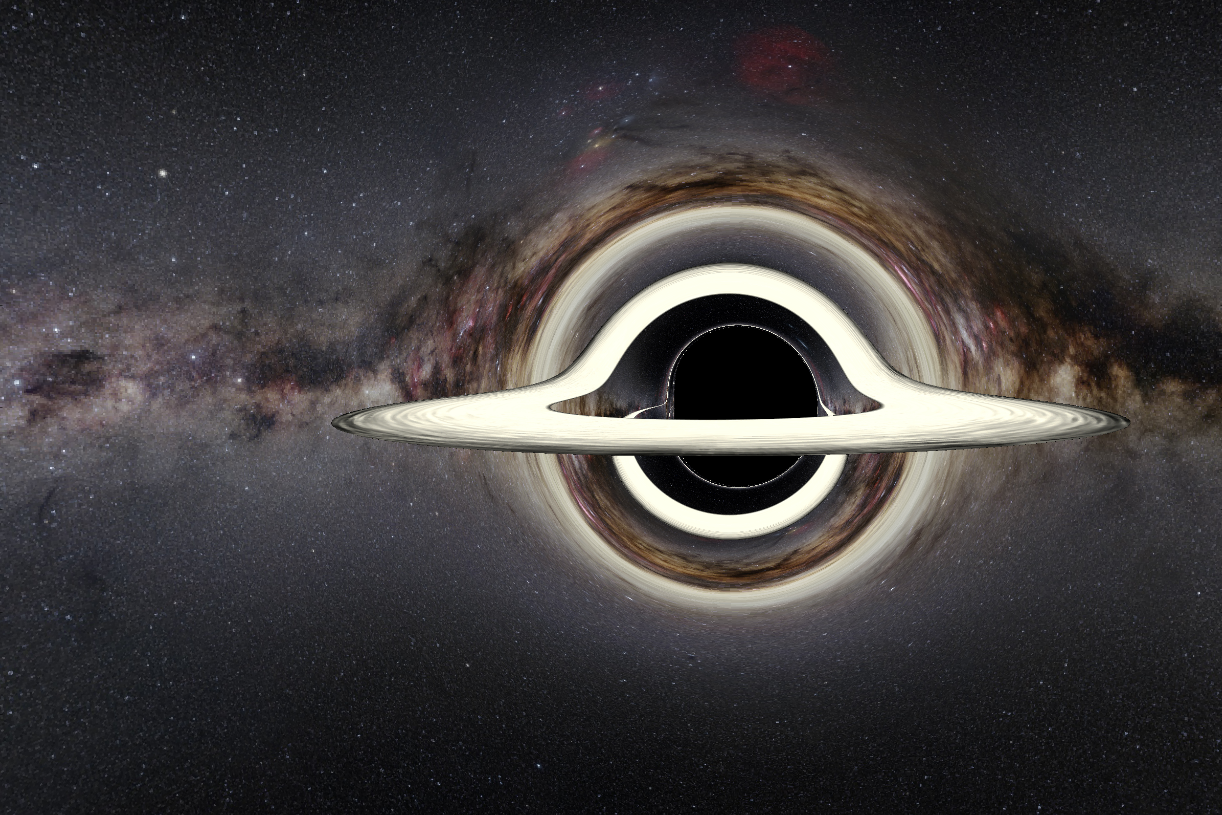
\includegraphics[width=\linewidth]{gfx/bh_texture_disk}
	\caption[Cinematographic textured image]{Cinematographic textured image}
	\label{fig:blackhole}
\end{figure}

Furthermore, the implemented \ac{ODE} solver accuracy was successfully tested, while the speed up of the \ac{GPU} parallelized code was proved to be very high.

\section{Ray Tracer Features}

The ray tracer generates images with a wide range of possibilities. First of all, it can render images that simulate photographies made with a common camera near the black hole. An accretion disk can be added to the black hole, showing the curvature of the light near its surroundings. For both the disk and the celestial sphere, arbitrary textures can be added, letting the user experiment with the light and the distortions produced by the greatly curved spacetime near the Kerr black hole.

\begin{figure}[bth]
	\myfloatalign
	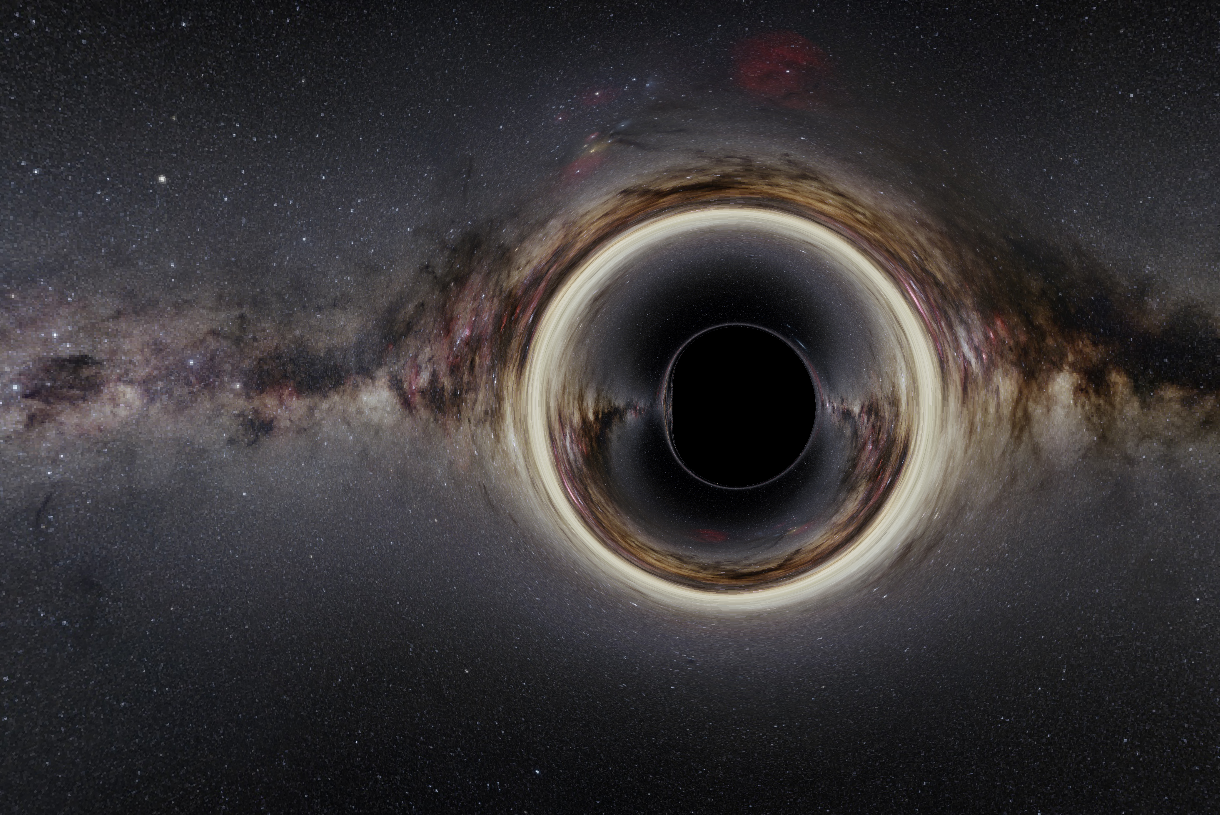
\includegraphics[width=\linewidth]{gfx/bh_texture_nodisk}
	\caption[Textured image without accretion disk]{Textured image without accretion disk}
	\label{fig:blackholenodisk}
\end{figure}

\autoref{fig:blackhole} is one example of a fully featured image with a cinematographic look: the celestial sphere is textured with an image of the Milky Way; an accretion disk around the black hole is added and a texture on the disk is rendered.

\autoref{fig:blackholenodisk} shows the same previous image, but rendered without the disk to better see the distortion produced by the black hole.

Furthermore, the rendered images can be plotted as three dimensional projections, letting the user observe the paths followed by the geodesics in order to understand how they were curved.

An example of this feature can be seen on \autoref{fig:3dprojection}, where four snapshots of the three dimensional projection are shown. Blue lines represent geodesics that come from the celestial sphere, red lines are geodesics that never existed, as they would have originated inside the black hole's horizon; finally, the green lines are the geodesics whose origin is on the accretion disk.

The computed information can rendered independently as a three dimensional projection or as an image. \autoref{fig:3dprojectionimage} shows the photography whose three dimensional representation was depicted on \autoref{fig:3dprojection}. In this case, the disk is textured with a coloured patched texture.

\begin{figure}[bth]
	\myfloatalign
	\subfloat[Top view.]
	{\frame{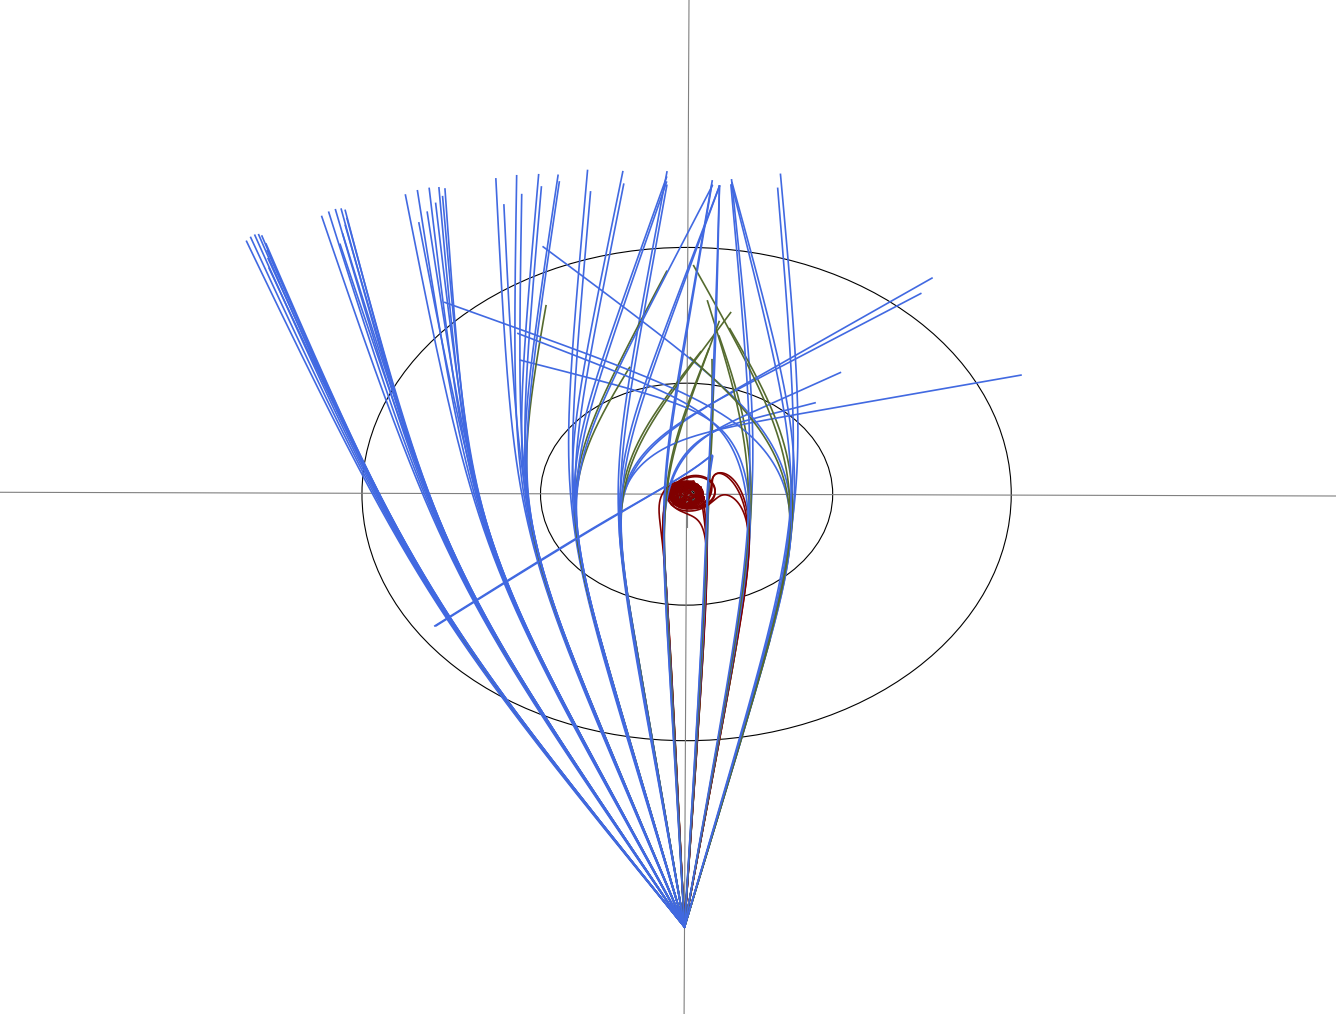
\includegraphics[width=.45\linewidth]{gfx/3d_01_top}}} \quad
	\subfloat[Right view.]
	{\frame{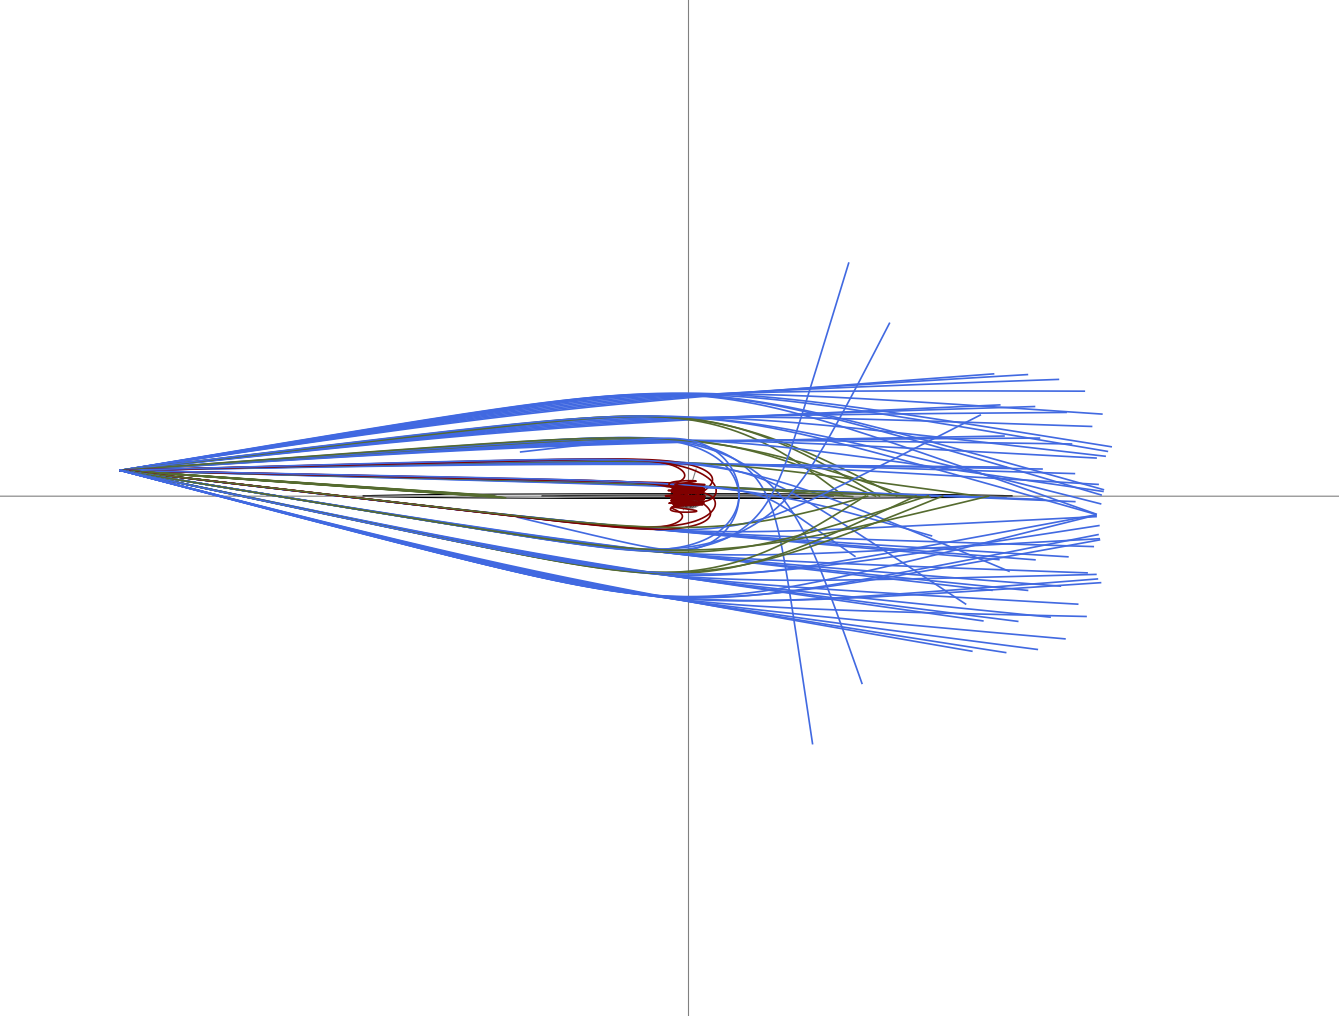
\includegraphics[width=.45\linewidth]{gfx/3d_01_right}}} \\
	\subfloat[Perspective view from behind.]
	{\frame{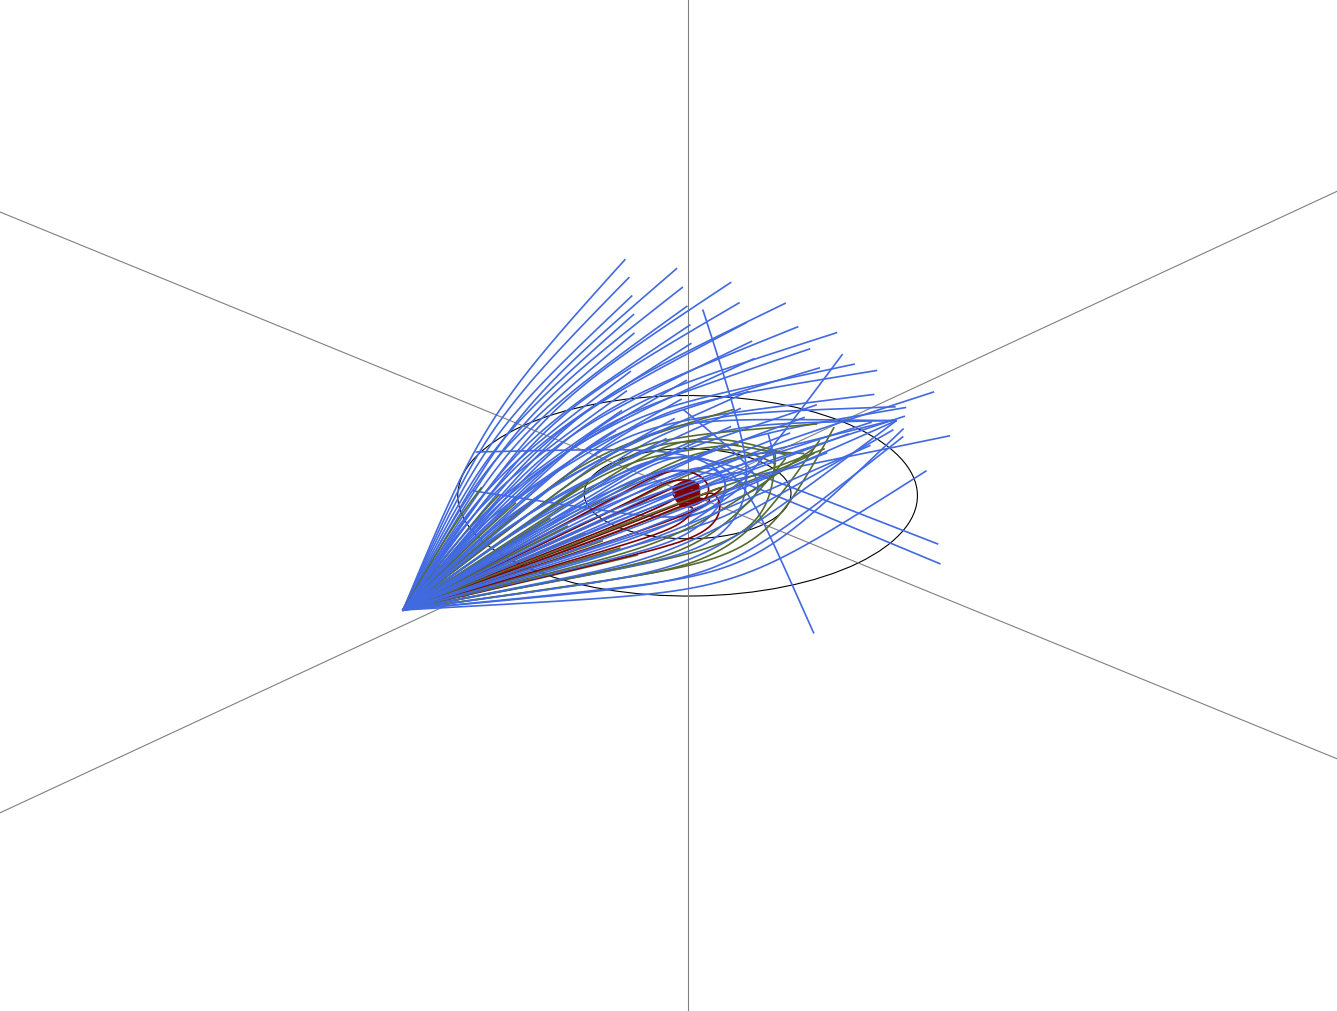
\includegraphics[width=.45\linewidth]{gfx/3d_01_perspective1}}} \quad
	\subfloat[Perspective view from the front side.]
	{\frame{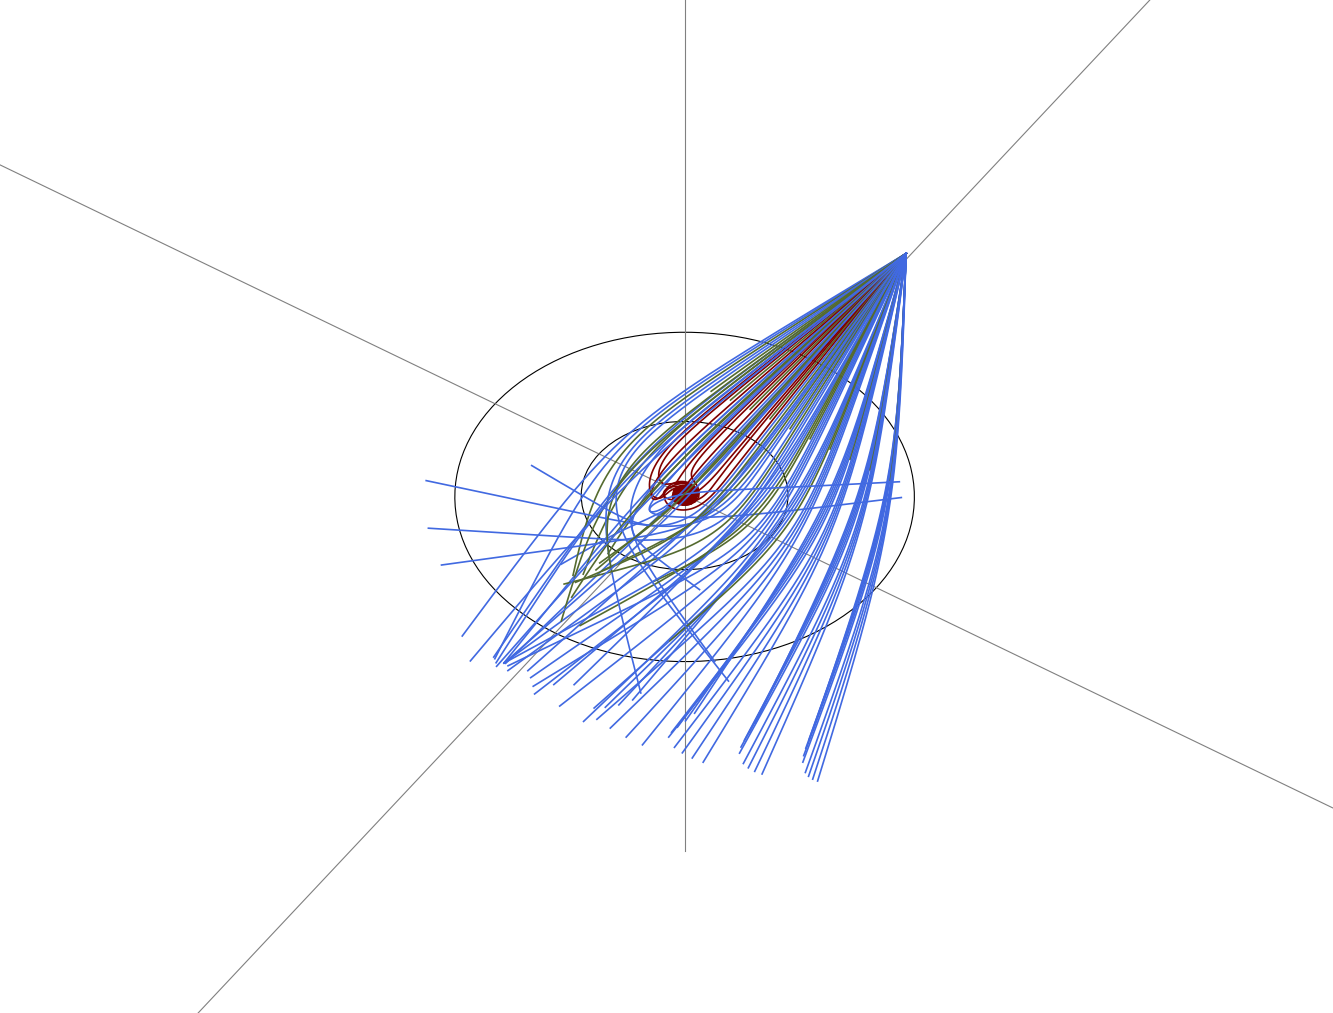
\includegraphics[width=.45\linewidth]{gfx/3d_01_perspective2}}}
	\caption[3D representation of the geodesics]{3D representation of the geodesics.}\label{fig:3dprojection}
\end{figure}

\begin{figure}[bth]
	\myfloatalign
	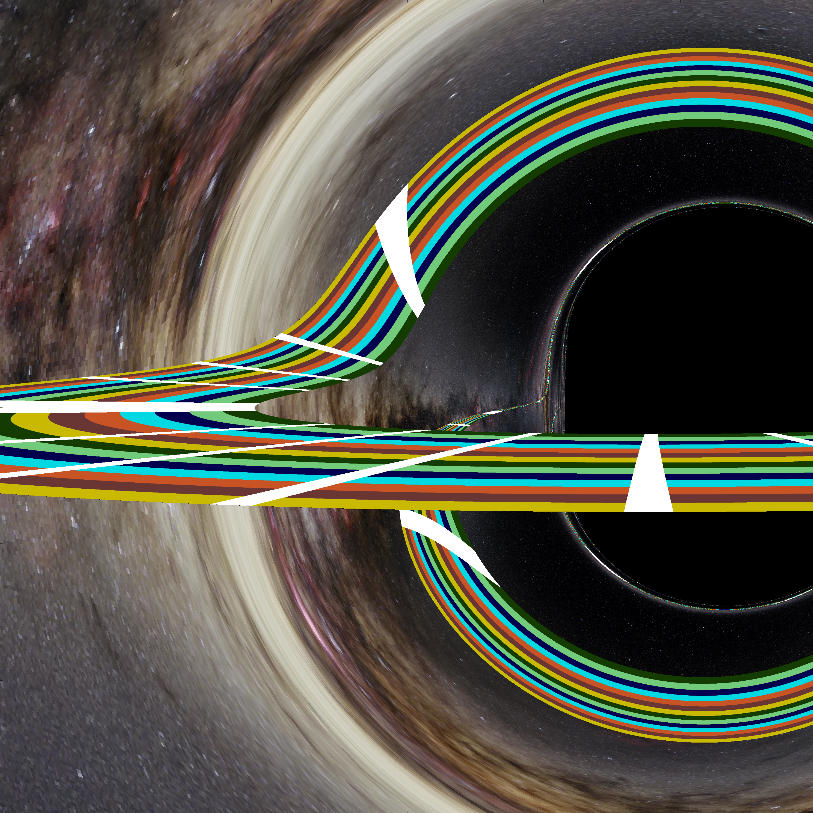
\includegraphics[width=.7\linewidth]{gfx/3d_01_image}
	\caption[Photography from a 3D scenario]{Photography of the 3D scenario rendered in \autoref{fig:3dprojection}}
	\label{fig:3dprojectionimage}
\end{figure}

\section{Computational Results}

This section covers the computational results of the implemented code; \ie, it studies the accuracy and efficiency of the ray tracer.

\subsection{Runge-Kutta Solver Accuracy}

The \ac{RK} solver has been tested not only against the geodesics \ac{ODE} system, but against usual functions whose analytic expression is known. This basic test was done with two purposes:
\begin{enumerate}
	\item To test that the solver was accurate.
	\item To study the behaviour of the automatic step size computation.
\end{enumerate}

One example of this test can be seen on \autoref{fig:stepsize}, that shows the behaviour of the \ac{RK} solver on the Airy function $Bi(x)$. The orange line is its analytic expression, which is
\[
	Bi(x) = \frac{1}{\pi} \int_0^\infty \cos\left(\frac{t^3}{3} + xt\right)dt,
\]
while the blue points are the solution computed by the \ac{RK} solver of the \ac{ODE} whose solution is $Bi(x)$, that is
\[
	\frac{d^2y}{dx^2} - xy = 0.
\]

\begin{figure}[bth]
	\myfloatalign
	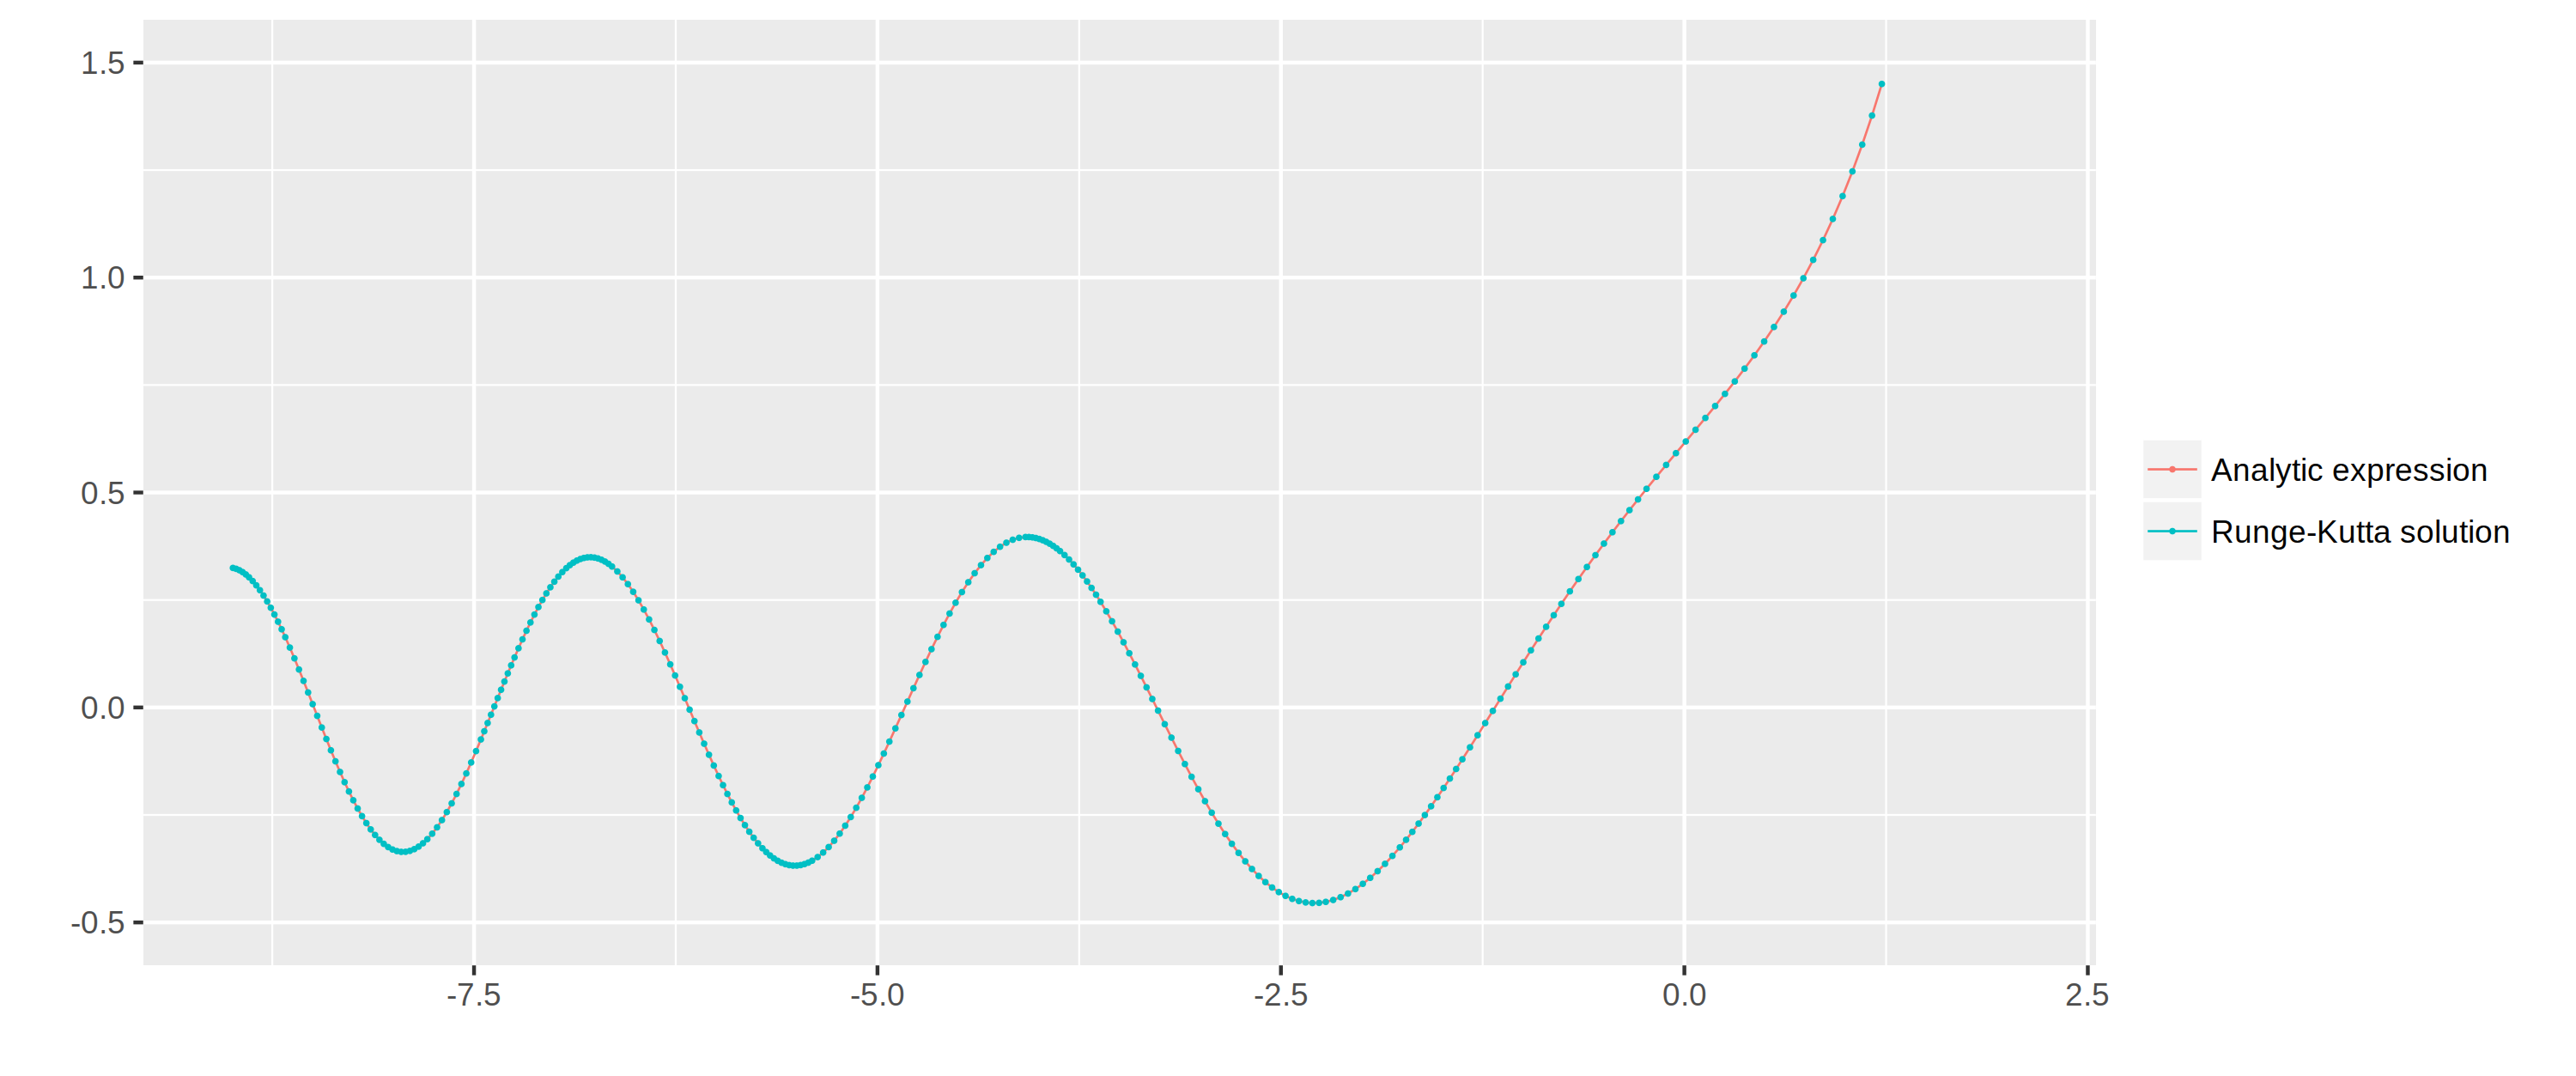
\includegraphics[width=1.3\linewidth]{gfx/analytic}
	\caption[Solver in an analytic function]{\ac{RK} solver in an analytic function}
	\label{fig:stepsize}
\end{figure}

It can be seen how the automatic step computation algorithm works smoothly: when the function can be approximated as a straight line, the step, which is the space between successive points, is very large. However, in intervals where the function changes rapidly its curvature, the algorithm reduces the step in order to better approximate the function value.

\begin{figure}[bth]
	\myfloatalign
	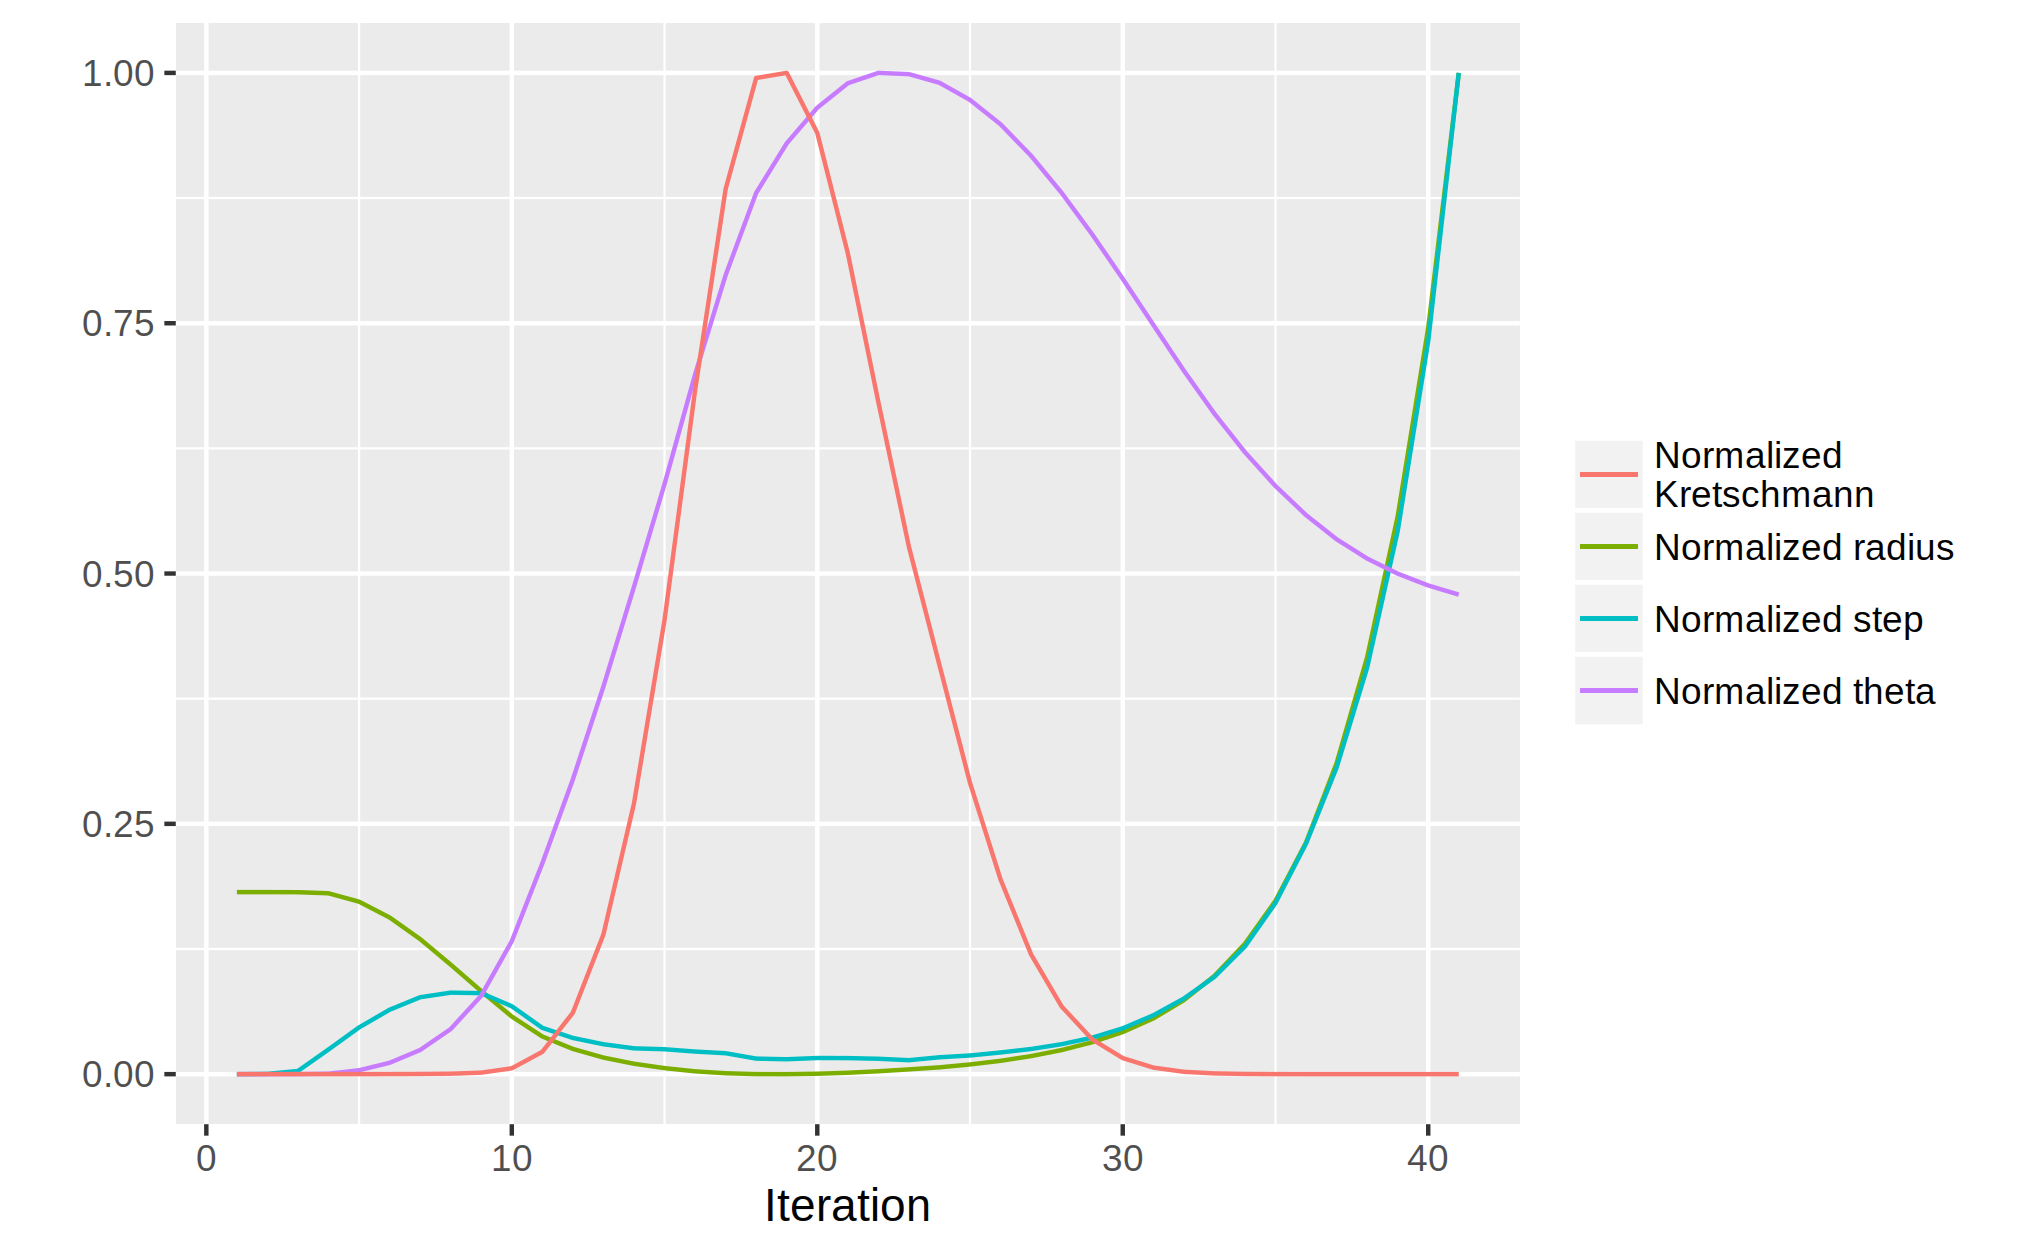
\includegraphics[width=1.2\linewidth]{gfx/kretschmann}
	\caption[Step, $r$, $\vartheta$ and Kretschmann]{Step, radius, $\vartheta$ and Kretschmann}
	\label{fig:kretschmann}
\end{figure}

This behaviour can also be seen on the geodesics \ac{ODE} system. \autoref{fig:kretschmann} shows the normalized values of four quantities:
\begin{enumerate}
	\item The Kretschmann invariant, which measures the curvature of the spacetime, and which is known to diverge in the singularity.
	\item The distance to the black hole.
	\item The value of the $\vartheta$ angle.
	\item The step computed by the automatic step algorithm.
\end{enumerate}

When the lightlike particle approaches the black hole; \ie, when the distance to the black hole decreases and, as a consequence, the Kretschmann increases, the system becomes unstable, and so the algorithm reduces the step size in order to better approximate its value.

In fact, both the step line and the radius line are very similar, showing the correlation between the computed step and the distance to the black hole centre.

\subsection{Efficiency}

Regarding the efficiency of the ray tracer, a benchmark against a \ac{CPU} implementation has been done.

The \ac{CPU} implementation has essentially the same code that the \ac{GPU}-parallelized version, except for the obvious changes that were made to adapt the code to the \ac{CUDA} grid.

\autoref{fig:speedup} shows two benchmarks using both versions of the ray tracer: one with a Kerr spacetime where the black hole has a spin of $a = 0.0001$ and another one where the spin is $a = 0.999$.

For both benchmarks, the speed up is plotted, \ie, the line represented for each of them shows how many times faster is the \ac{GPU}-parallelized version against the \ac{CPU} implementation.

\begin{figure}[bth]
	\myfloatalign
	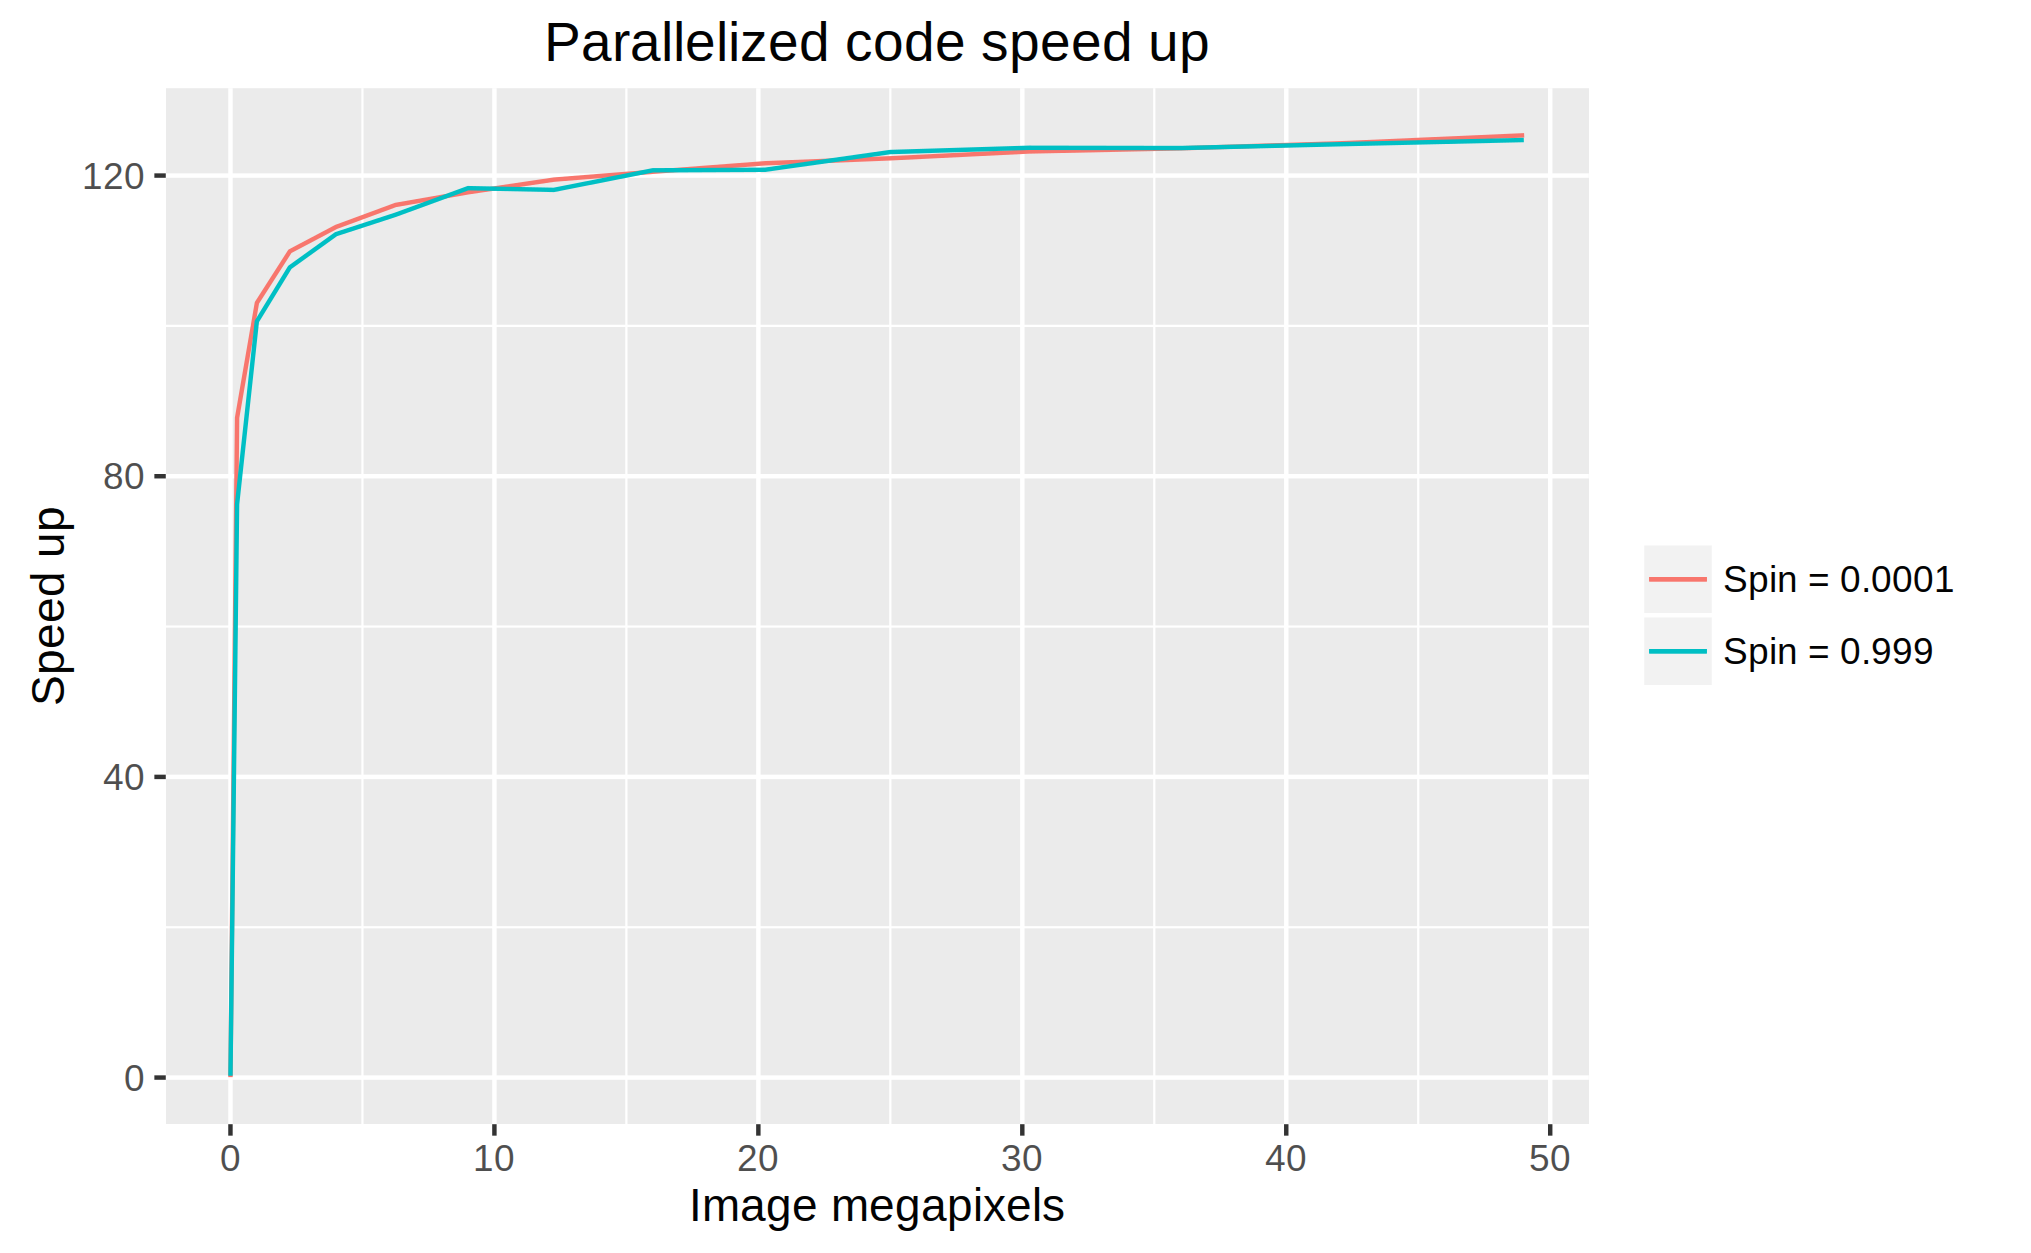
\includegraphics[width=1.2\linewidth]{gfx/speedup}
	\caption[Speed up with different spins]{Speed up with different spins}
	\label{fig:speedup}
\end{figure}

The speed up increases at a great speed when the number of pixels are augmented. It stabilizes around 20 megapixels with a speed up of about $125$. The mean speed up equals $108.5$ on the low spin case, whereas in the high spin case equals $107.2$. The maximum speedup obtained equals $125.3$ on the first case, with a maximum speed up of $124.7$ on the second.

As we can see, these numbers do not vary too much depending on the spin, so the speed up seems to be stable against these changes. This figure summarises the power of the \ac{GPGPU}, that can increase the performance of a piece of software by several orders of magnitude.


\section{Scientific Results}

The main objective of the ray tracer implementation was to serve as a tool for scientists to study properties of the Kerr spacetime. This section summarises some of these interesting features.

\subsection{Spin}

The effect of the black hole spin on its surroundings has been studied in two ways.

First of all, we have generated images without any accretion disk and without textures for the celestial sphere. This gives us binaries images where the black pixels represent the shadow of the black hole and the white pixels the geodesics that came from the celestial sphere.

\autoref{fig:shadow} shows four images taken with the same camera, which is placed on the equatorial plane, with a null speed and focusing the black hole's centre. The only change between images is the black hole's spin.

The first one shows a perfect sphere. This is the edge case where the Kerr metric can be reduced to the more simple Schwarzschild metric.

\autoref{fig:shadow-b} and \autoref{fig:shadow-c} shows the same image with an increased spin. There is a slight change on the virtual position of the shadow and, although it is difficult to see, the shape is not circular.

The edge case, depicted on \autoref{fig:shadow-d}, makes clear the effect of a large spin on the shadow of the black hole. As it curves the geodesics rapidly, it is seen slightly moved to the right and with a flat side on the left: if the spin were of this same magnitude but negative, the image would be vertically mirrored.

\begin{figure}[bth]
	\myfloatalign
	\subfloat[Spin $\approx$ 0]
	{\frame{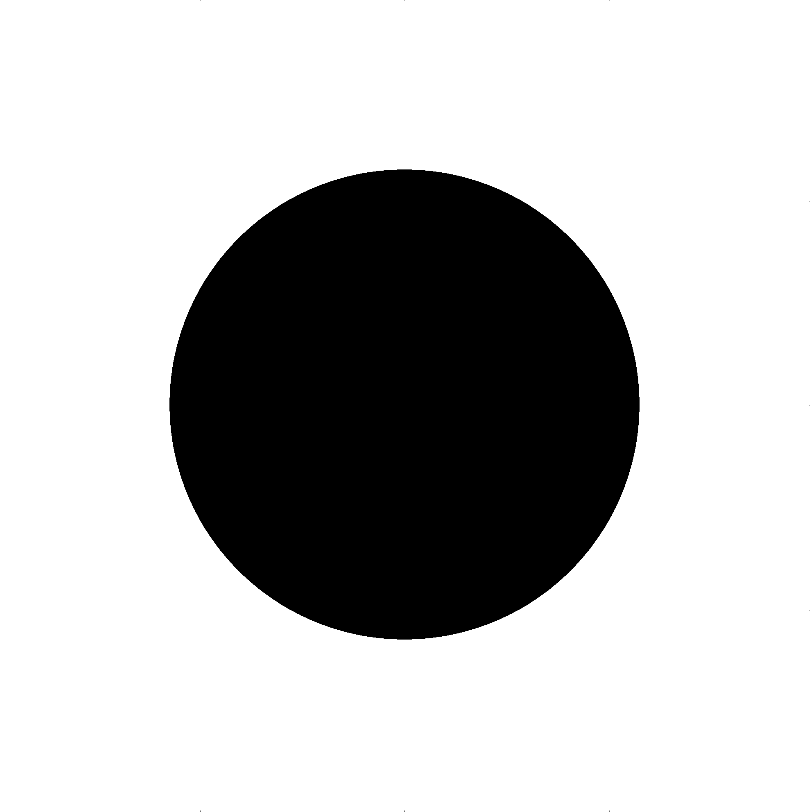
\includegraphics[width=.35\linewidth]{gfx/bh_shadow_spin0001}}} \quad
	\subfloat[Spin = 0.25]
	{\label{fig:shadow-b}%
		\frame{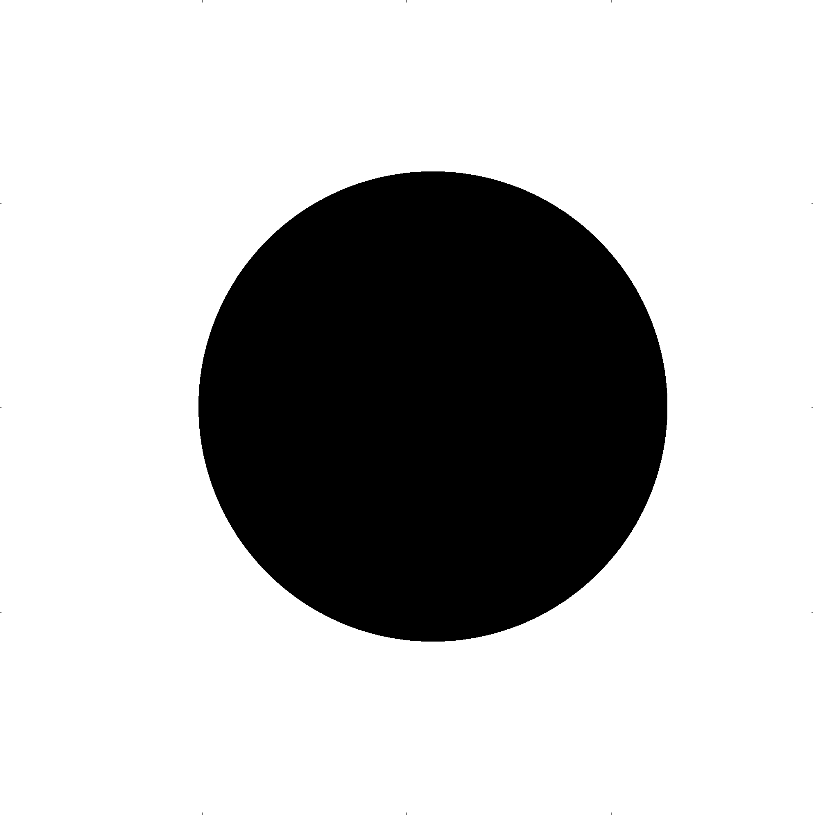
\includegraphics[width=.35\linewidth]{gfx/bh_shadow_spin25}}} \\
	\subfloat[Spin = 0.75]
	{\label{fig:shadow-c}%
		\frame{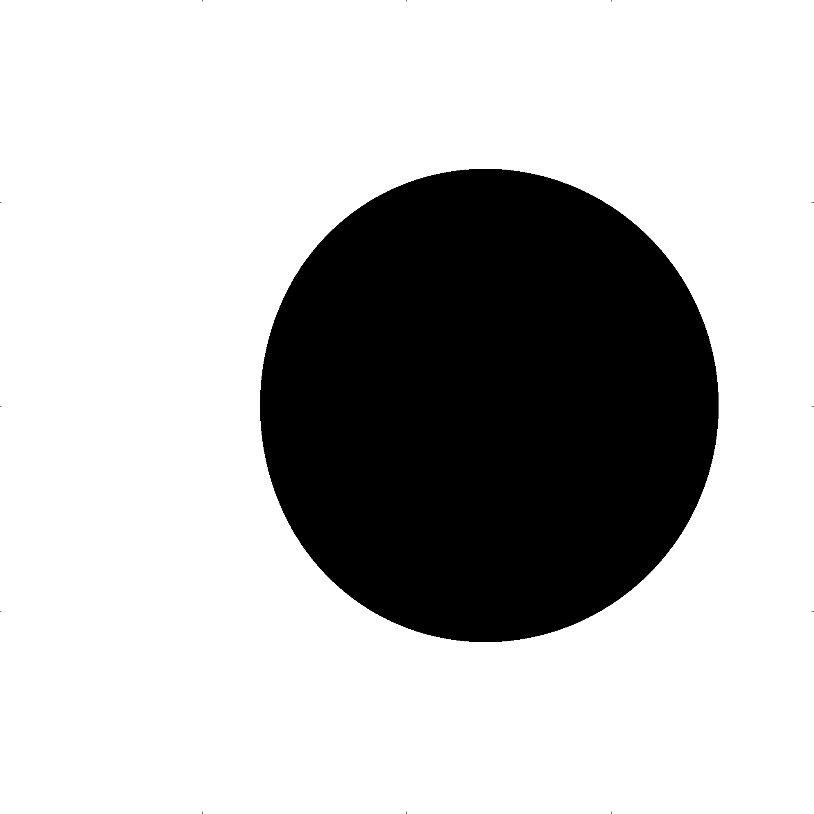
\includegraphics[width=.35\linewidth]{gfx/bh_shadow_spin75}}} \quad
	\subfloat[Spin $\approx$ 1]
	{\label{fig:shadow-d}%
		\frame{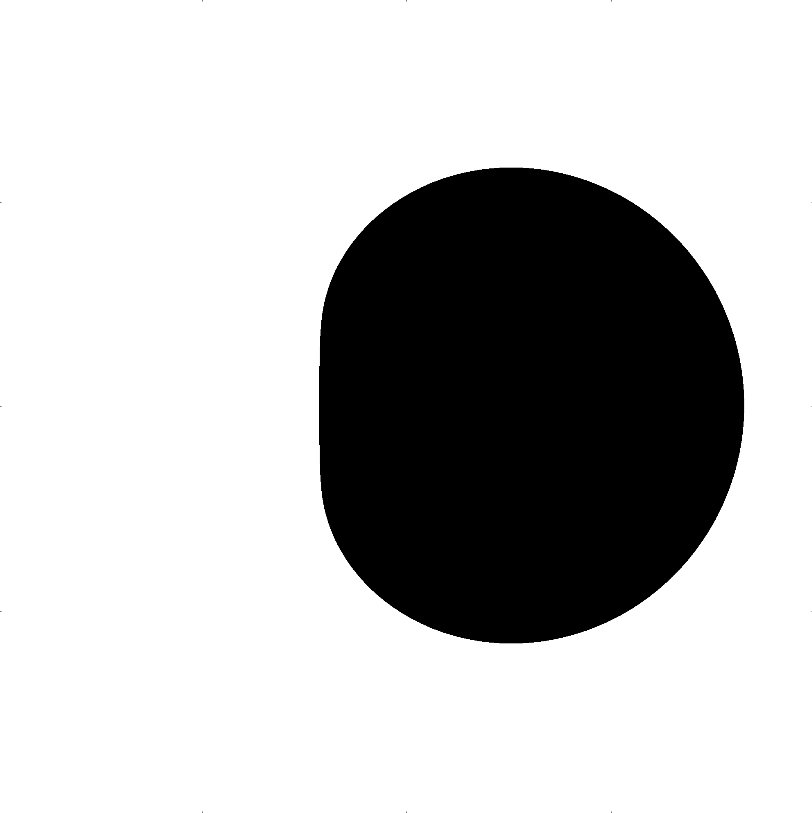
\includegraphics[width=.35\linewidth]{gfx/bh_shadow_spin999}}}
	\caption[Black hole shadow for different spins]{Black hole shadow for different spins}\label{fig:shadow}
\end{figure}

It is also interesting to see what happens with straight lines that fall inside the black hole.

Imagine an accretion disk around the black hole, with its inner radius minor than the horizon radius and an infinite outer radius. If we visualize this disk with a patched texture made by white and red squares, we can see the effect of the spin on its shape.

\autoref{fig:xmas-a} shows the most simple version of this scenario, where the black hole does not rotate: straight lines falling inside the black hole on the equatorial plane remain intact.

Taking this as the base case, we can see what happens when we increase the black hole's spin. \autoref{fig:xmas-b} and \autoref{fig:xmas-c} shows the scenario for spins of $0.25$ and $0.75$. The straight lines start to rotate accordingly with the black hole.

The most interesting image is depicted on \autoref{fig:xmas-d}, where we see an extreme spin of nearly 1. The lines curve greatly when they approach the shadow, and start rotating rapidly when they are close to the horizon.

\begin{figure}[bth]
	\myfloatalign
	\subfloat[Spin $\approx$ 0]
	{\label{fig:xmas-a}%
		\frame{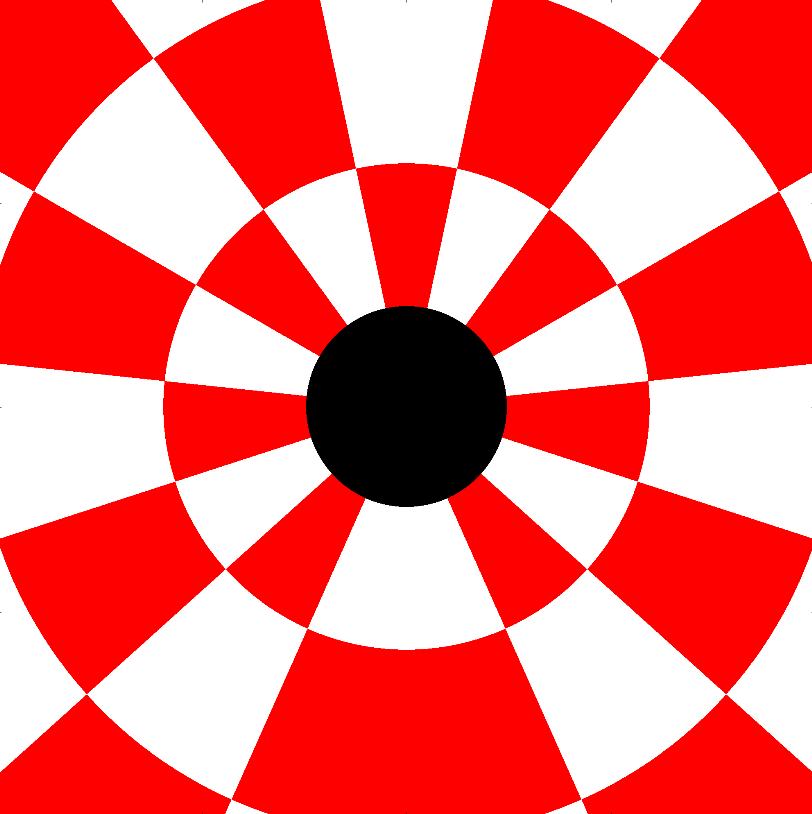
\includegraphics[width=.35\linewidth]{gfx/bh_xmas_spin0001}}} \quad
	\subfloat[Spin = 0.25]
	{\label{fig:xmas-b}%
		\frame{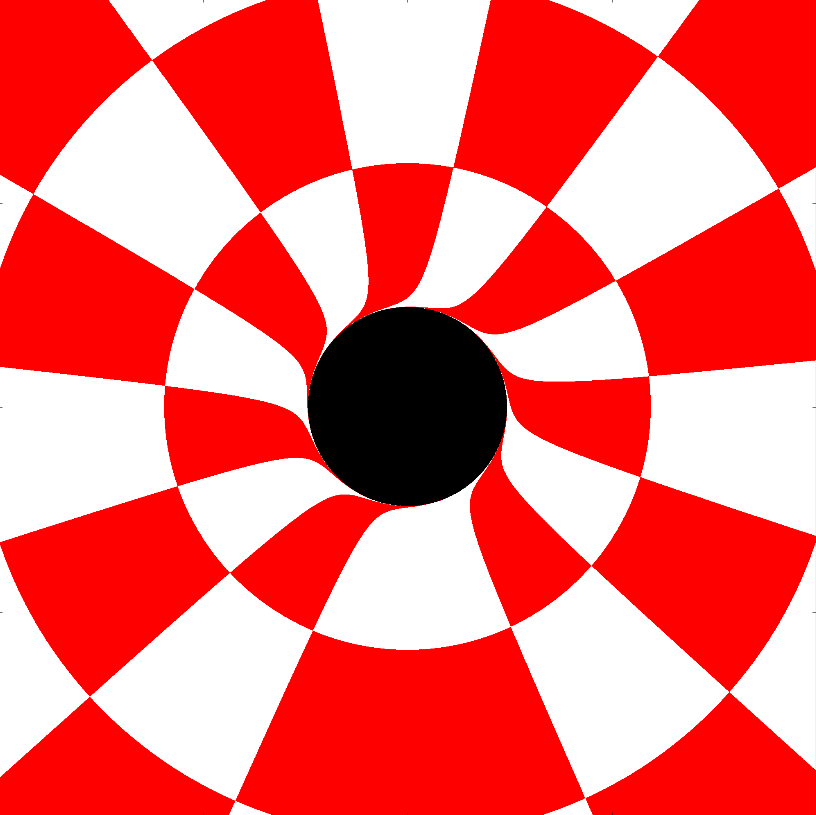
\includegraphics[width=.35\linewidth]{gfx/bh_xmas_spin25}}} \\
	\subfloat[Spin = 0.75]
	{\label{fig:xmas-c}%
		\frame{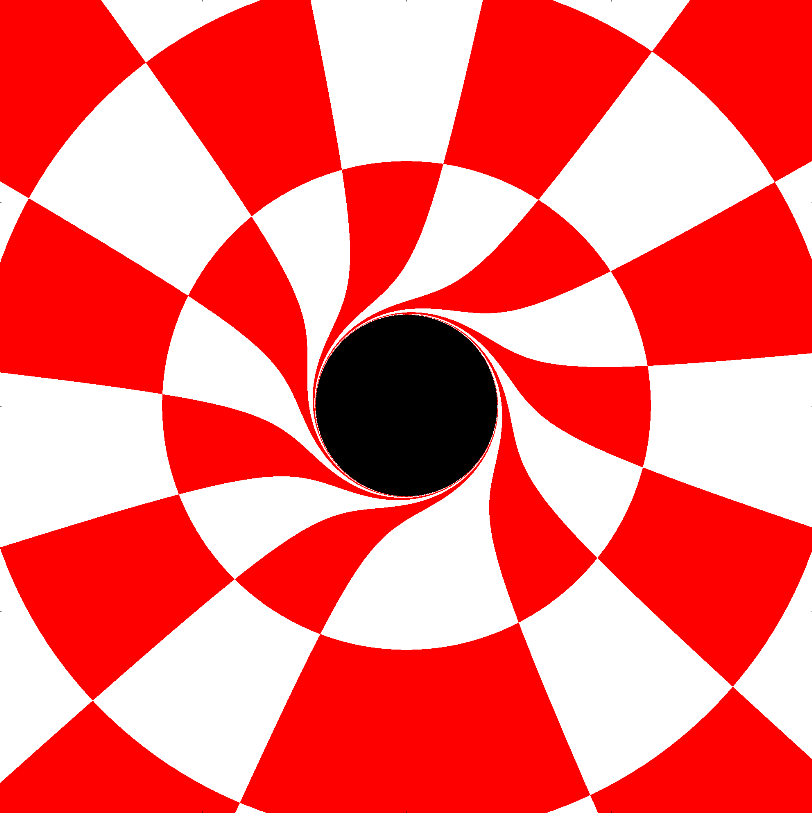
\includegraphics[width=.35\linewidth]{gfx/bh_xmas_spin75}}} \quad
	\subfloat[Spin $\approx$ 1]
	{\label{fig:xmas-d}%
		\frame{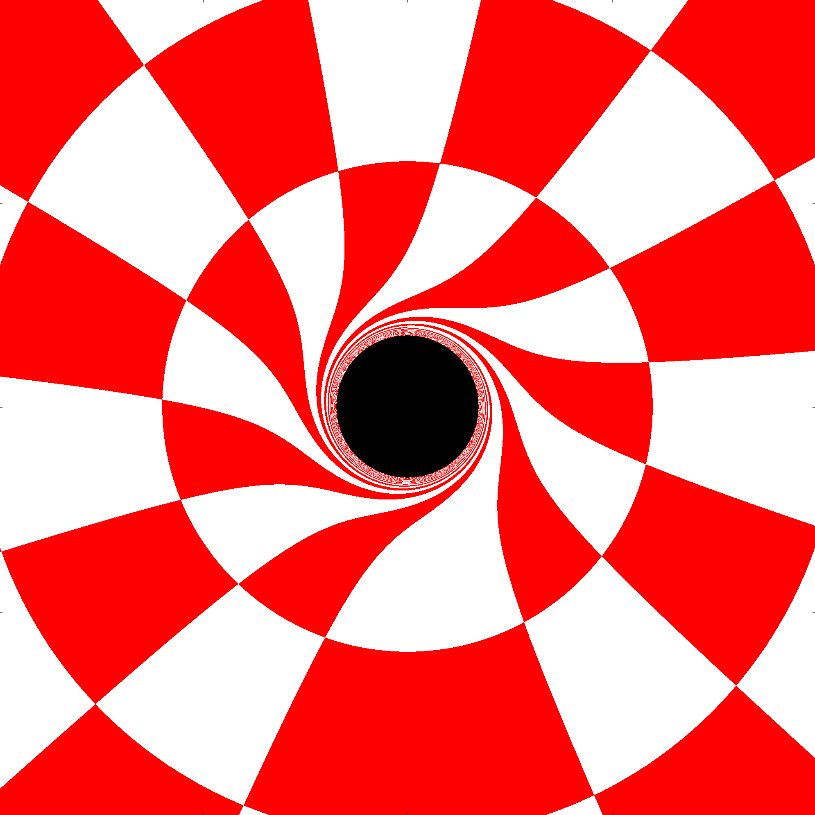
\includegraphics[width=.35\linewidth]{gfx/bh_xmas_spin999}}}
	\caption[Black hole shadow for different spins]{Black hole shadow for different spins}\label{fig:xmas}
\end{figure}

\subsection{Shadow}

One can map a texture on the black hole's horizon to really know what we are seeing when looking at the shadow.

\autoref{fig:texhoriz} shows such an image, where a patched texture drawing the meridians and the parallels has been mapped onto the horizon's surface.

This image tells us that, when we are looking at the shadow of a Kerr black hole, we are seeing the whole surface of the horizon, not just the side facing to us.

\begin{figure}[bth]
	\myfloatalign
	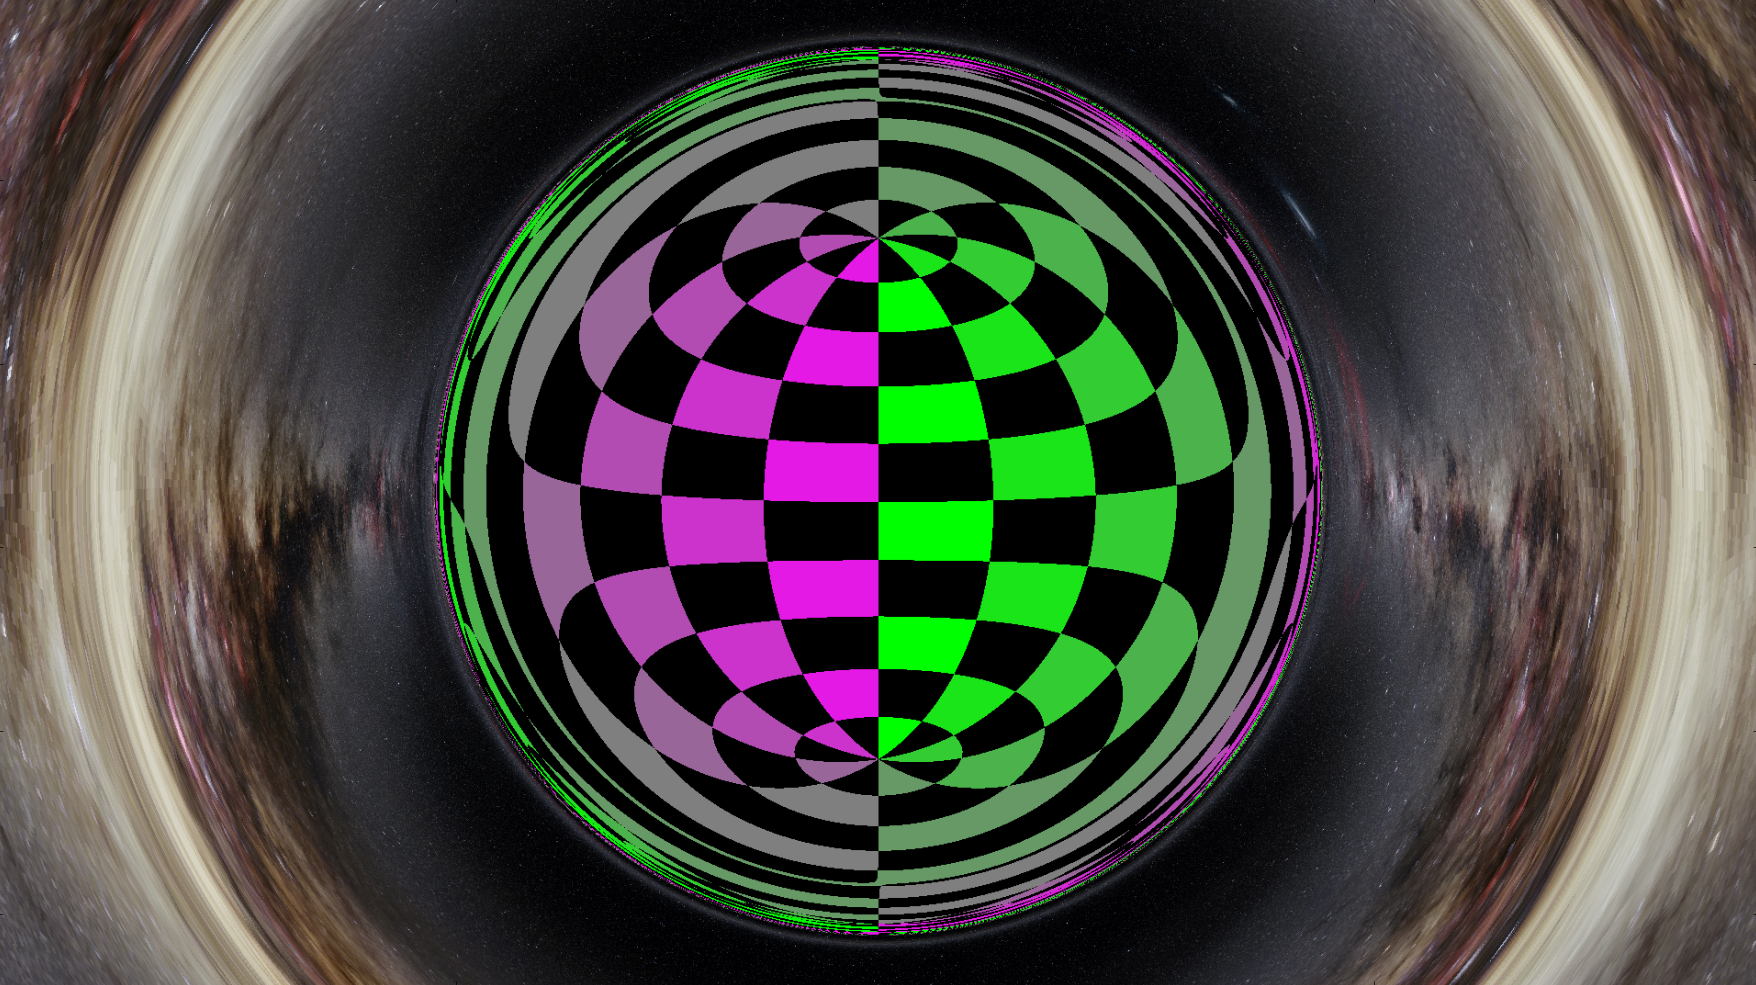
\includegraphics[width=.8\linewidth]{gfx/gridhorizon}
	\caption[Textured horizon]{Textured horizon.}
	\label{fig:texhoriz}
\end{figure}

\subsection{Accretion Disk}

\begin{figure}[bth]
	\myfloatalign
	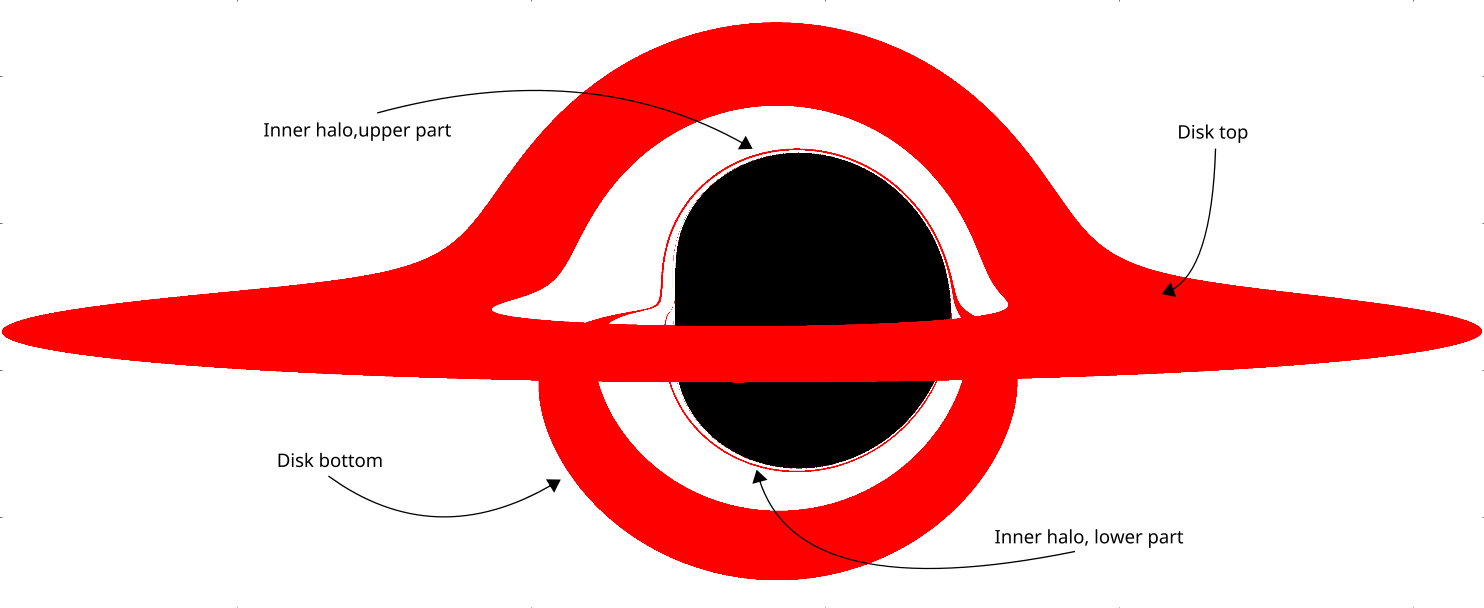
\includegraphics[width=\linewidth]{gfx/bh_simple}
	\caption[Accretion disk explained]{Accretion disk explained}
	\label{fig:explanation}
\end{figure}

The curvature of the disk around the black hole is really interesting. It let us understand the nature of the distortion produced by the spacetime.

Let us set up a simple image where the shadow is depicted with black pixels, the celestial sphere with white pixels and the disk with red ones.

\autoref{fig:explanation} shows this image, where we have noted the different parts of the disk we will talk about. The big stripe crossing the shadow that gets over it is the top of the disk. The lower stripe, that gets closer to the shadow and goes around on top of it is the disk bottom. We will denote the thin line just on top of the shadow as the upper part of the inner halo, where the thin line just below it will be called lower part of the inner halo.

It is interesting to visualize the geodesics that hit the disk in order to understand the processes that lead us to see the disk with such a great distortion.

First of all, we can describe the disk bottom: it is formed by lightlike particles that travel below the black hole and hit the disk just at the back of the shadow. A three dimensional projection of a set of these geodesics can be seen on \autoref{fig:under_disk}.

\begin{figure}[bth]
	\myfloatalign
	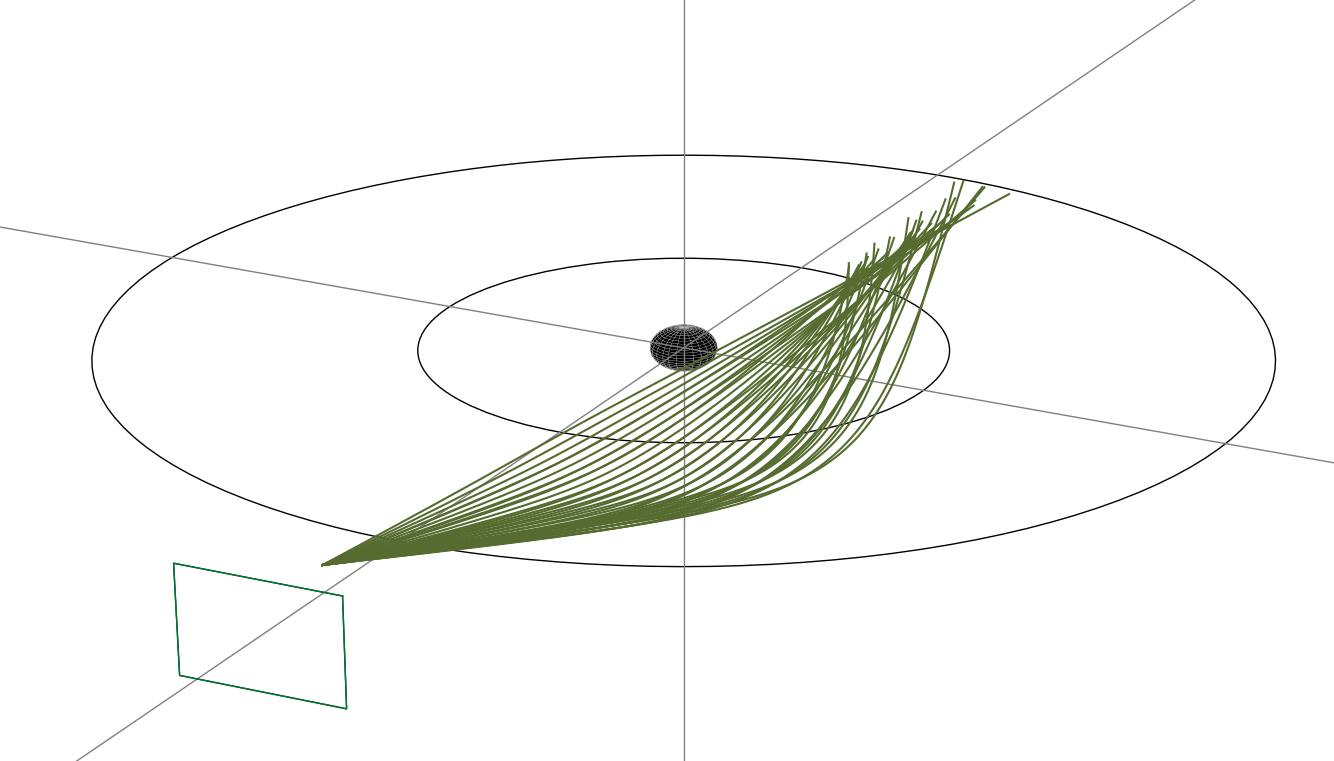
\includegraphics[width=.65\linewidth]{gfx/under_disk}
	\caption[Disk bottom]{Disk bottom.}
	\label{fig:under_disk}
\end{figure}

One of the most interesting parts of the disk distortion is the inner halo. \autoref{fig:insidehalo} shows a set of geodesics that formed its final image.

Furthermore, we can select the geodesics that form the upper part of the inner halo. \autoref{fig:upperhalo} shows the intricate paths followed by these geodesics, that twist around the black hole, get behind the disk and scatter to cover a great part of the bottom part of the disk.

\autoref{fig:wholehalo} summarises all this tour by plotting all geodesics that form the inner halo in just one image.

\begin{figure}[bth]
	\myfloatalign
	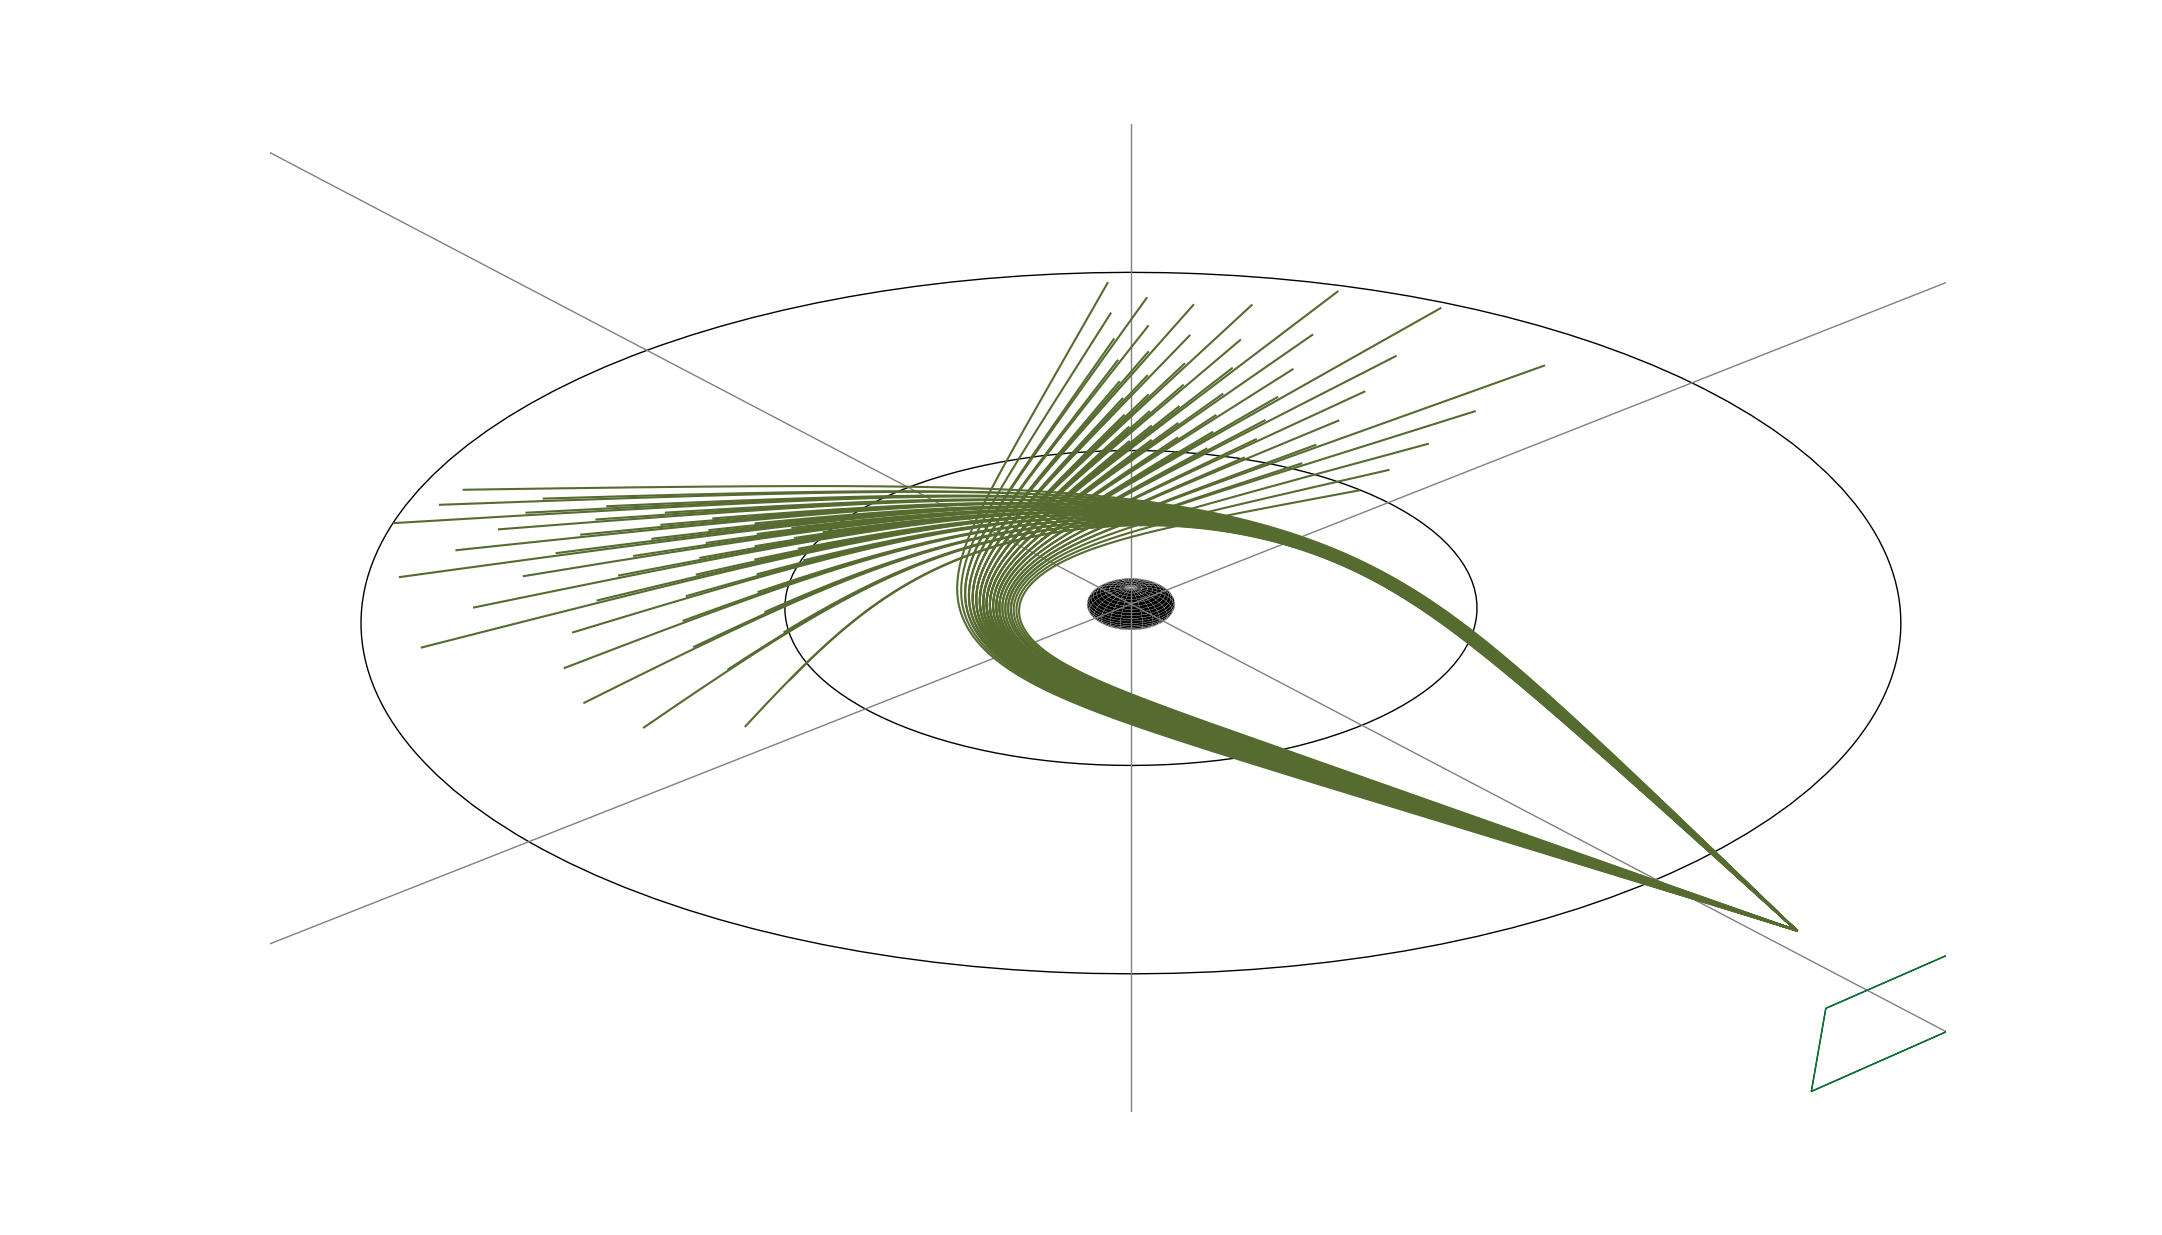
\includegraphics[width=.6\linewidth]{gfx/disk_inside_halo}
	\caption[Inner halo]{Inner halo.}
	\label{fig:insidehalo}
\end{figure}

\begin{figure}[bth]
	\myfloatalign
	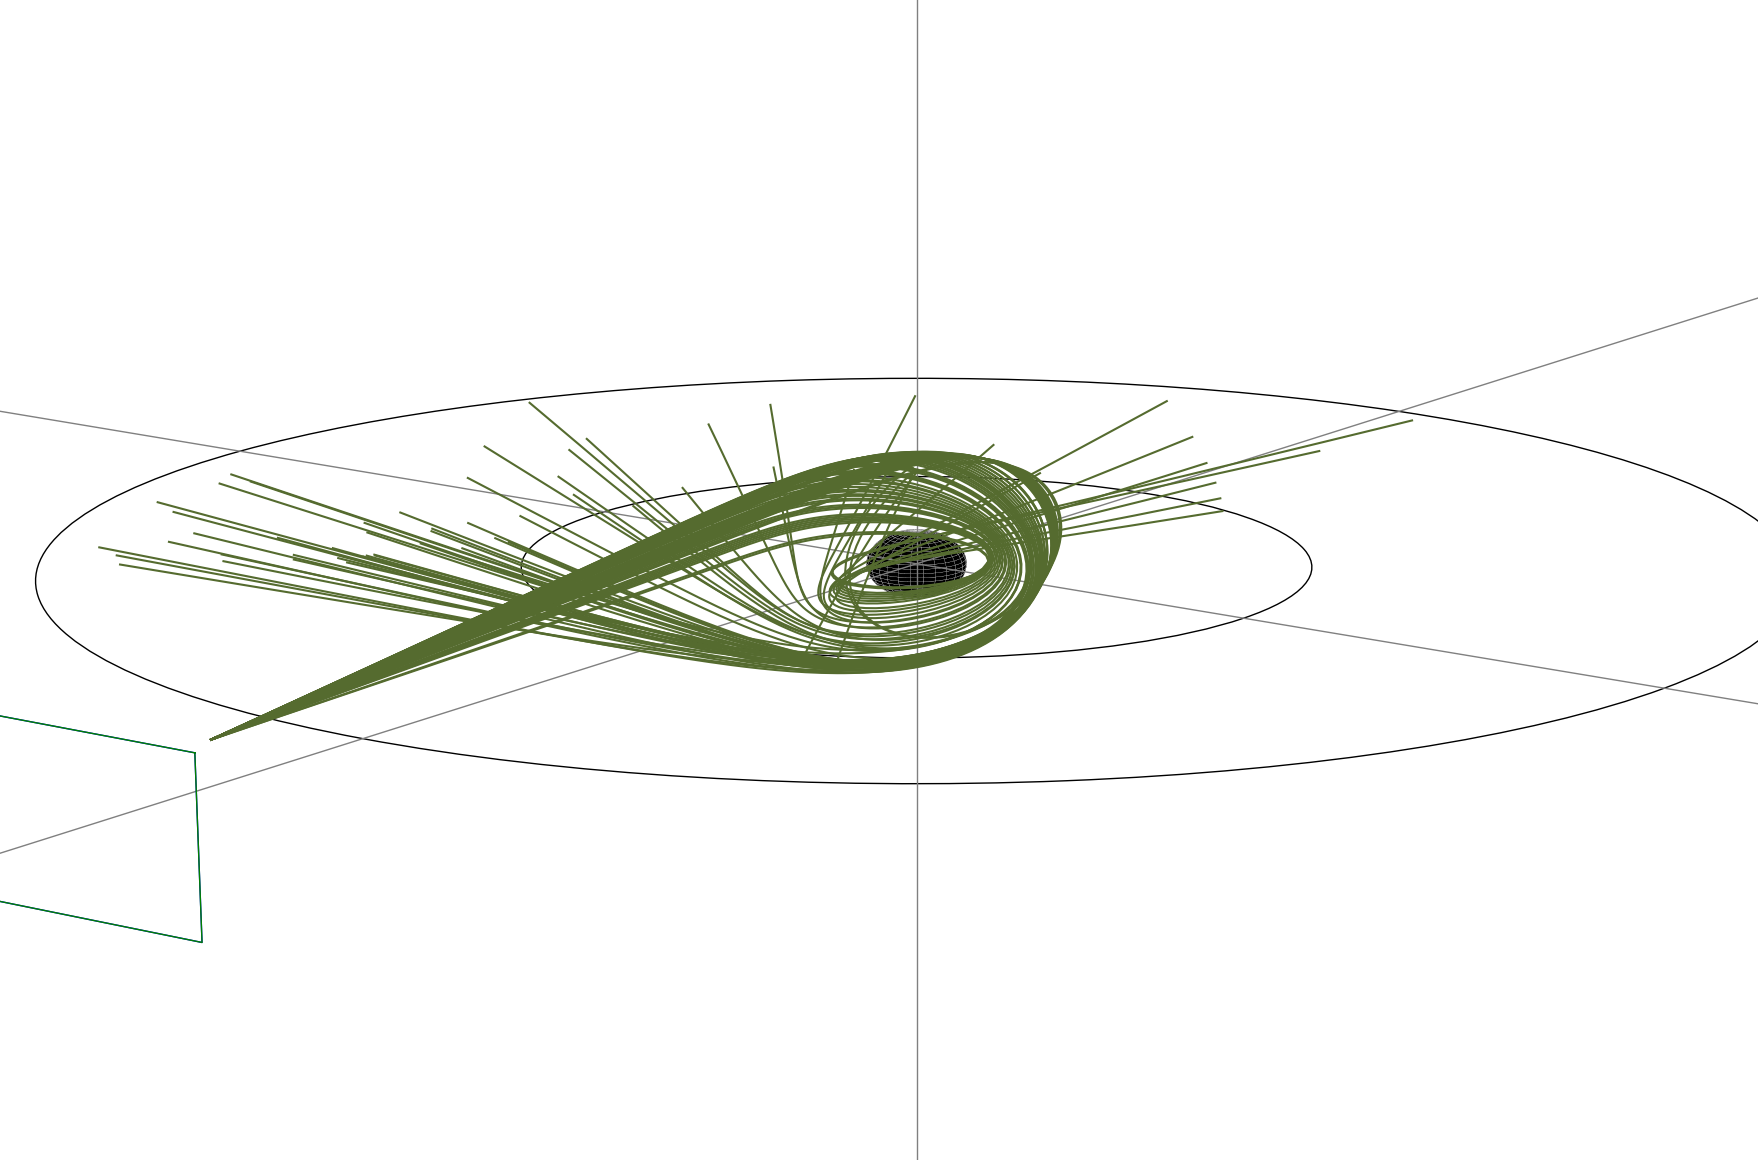
\includegraphics[width=.6\linewidth]{gfx/disk_inside_halo_superior}
	\caption[Upper part of the inner halo]{Upper part of the inner halo.}
	\label{fig:upperhalo}
\end{figure}

\begin{figure}[bth]
	\myfloatalign
	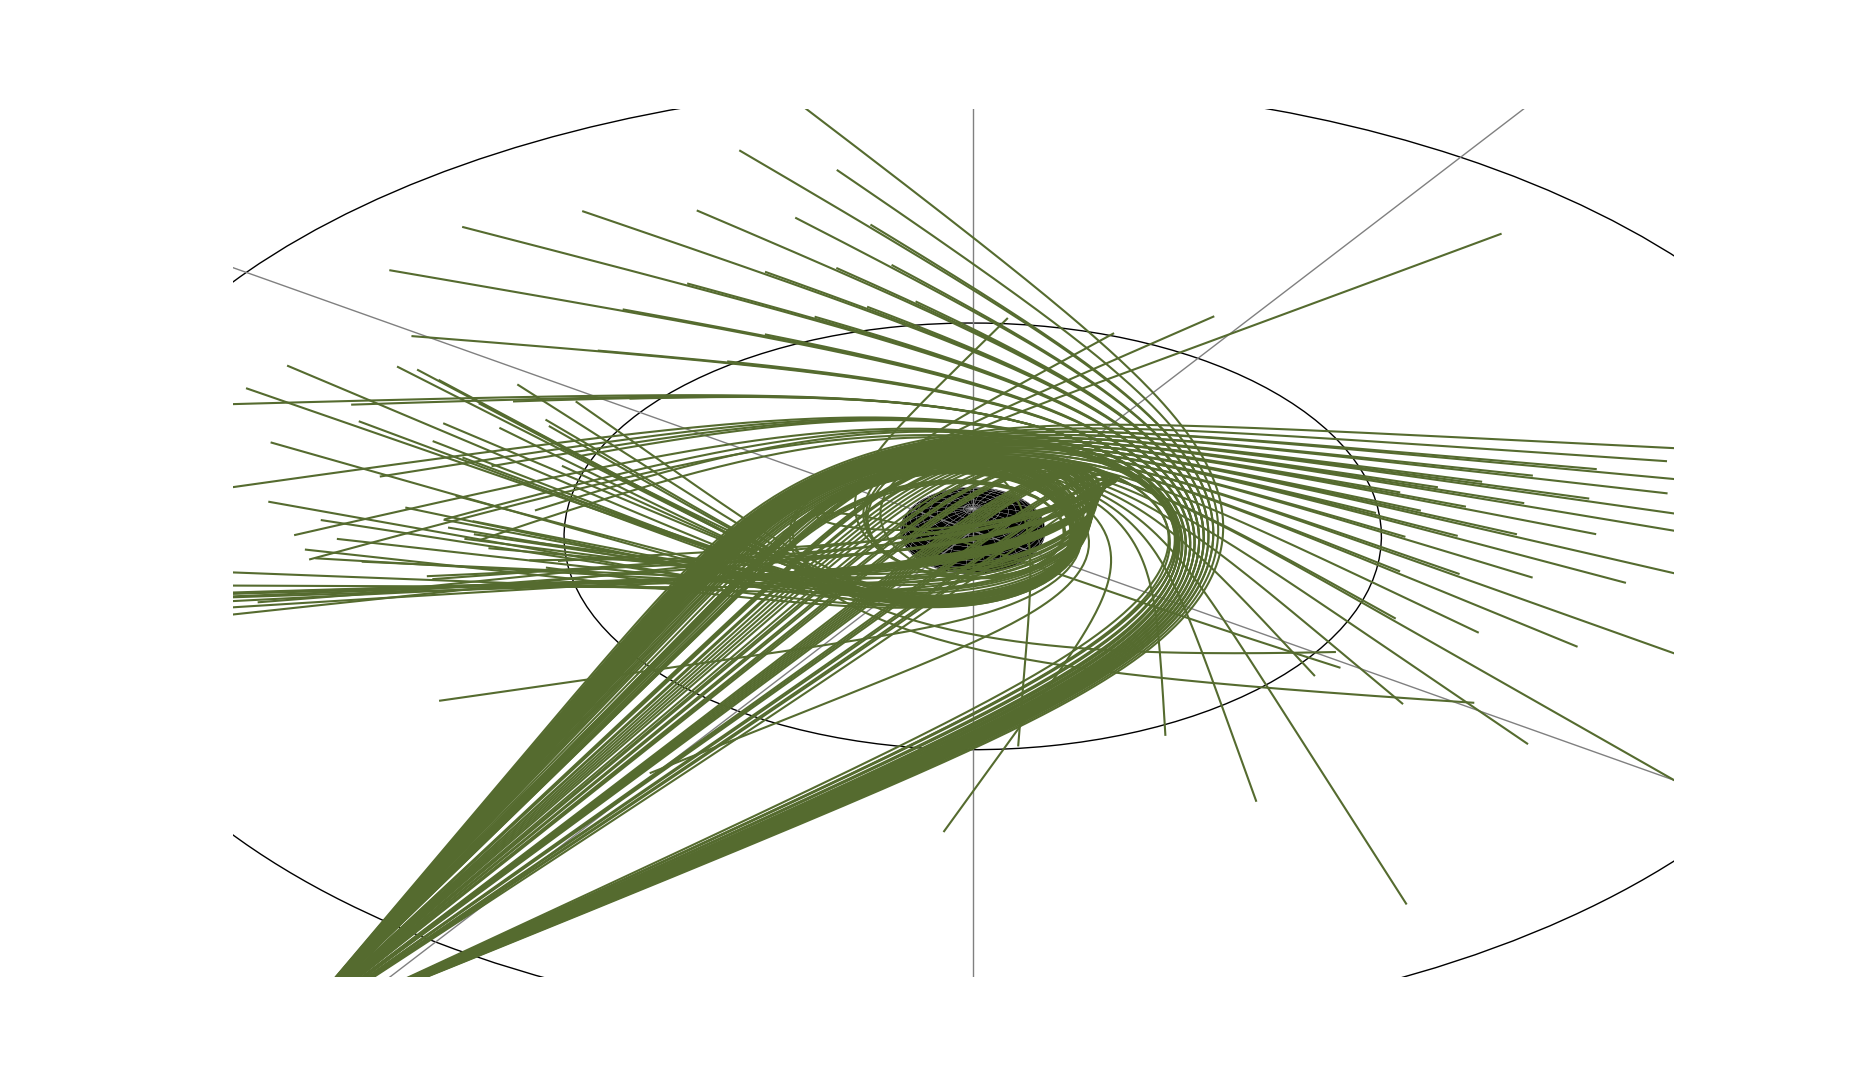
\includegraphics[width=.5\linewidth]{gfx/halo_entero}
	\caption[Geodesics forming the disk image]{Geodesics forming the disk image.}
	\label{fig:wholehalo}
\end{figure}

We can visualize, on the disk, the final point of the geodesic on the camera. In \autoref{fig:cathegories}, the black points represent the inner halo, the red points belong to the disk bottom, the green ones to the disk top and, finally, the blue points are the lower big stripe of the bottom disk.

\begin{figure}[bth]
	\myfloatalign
	{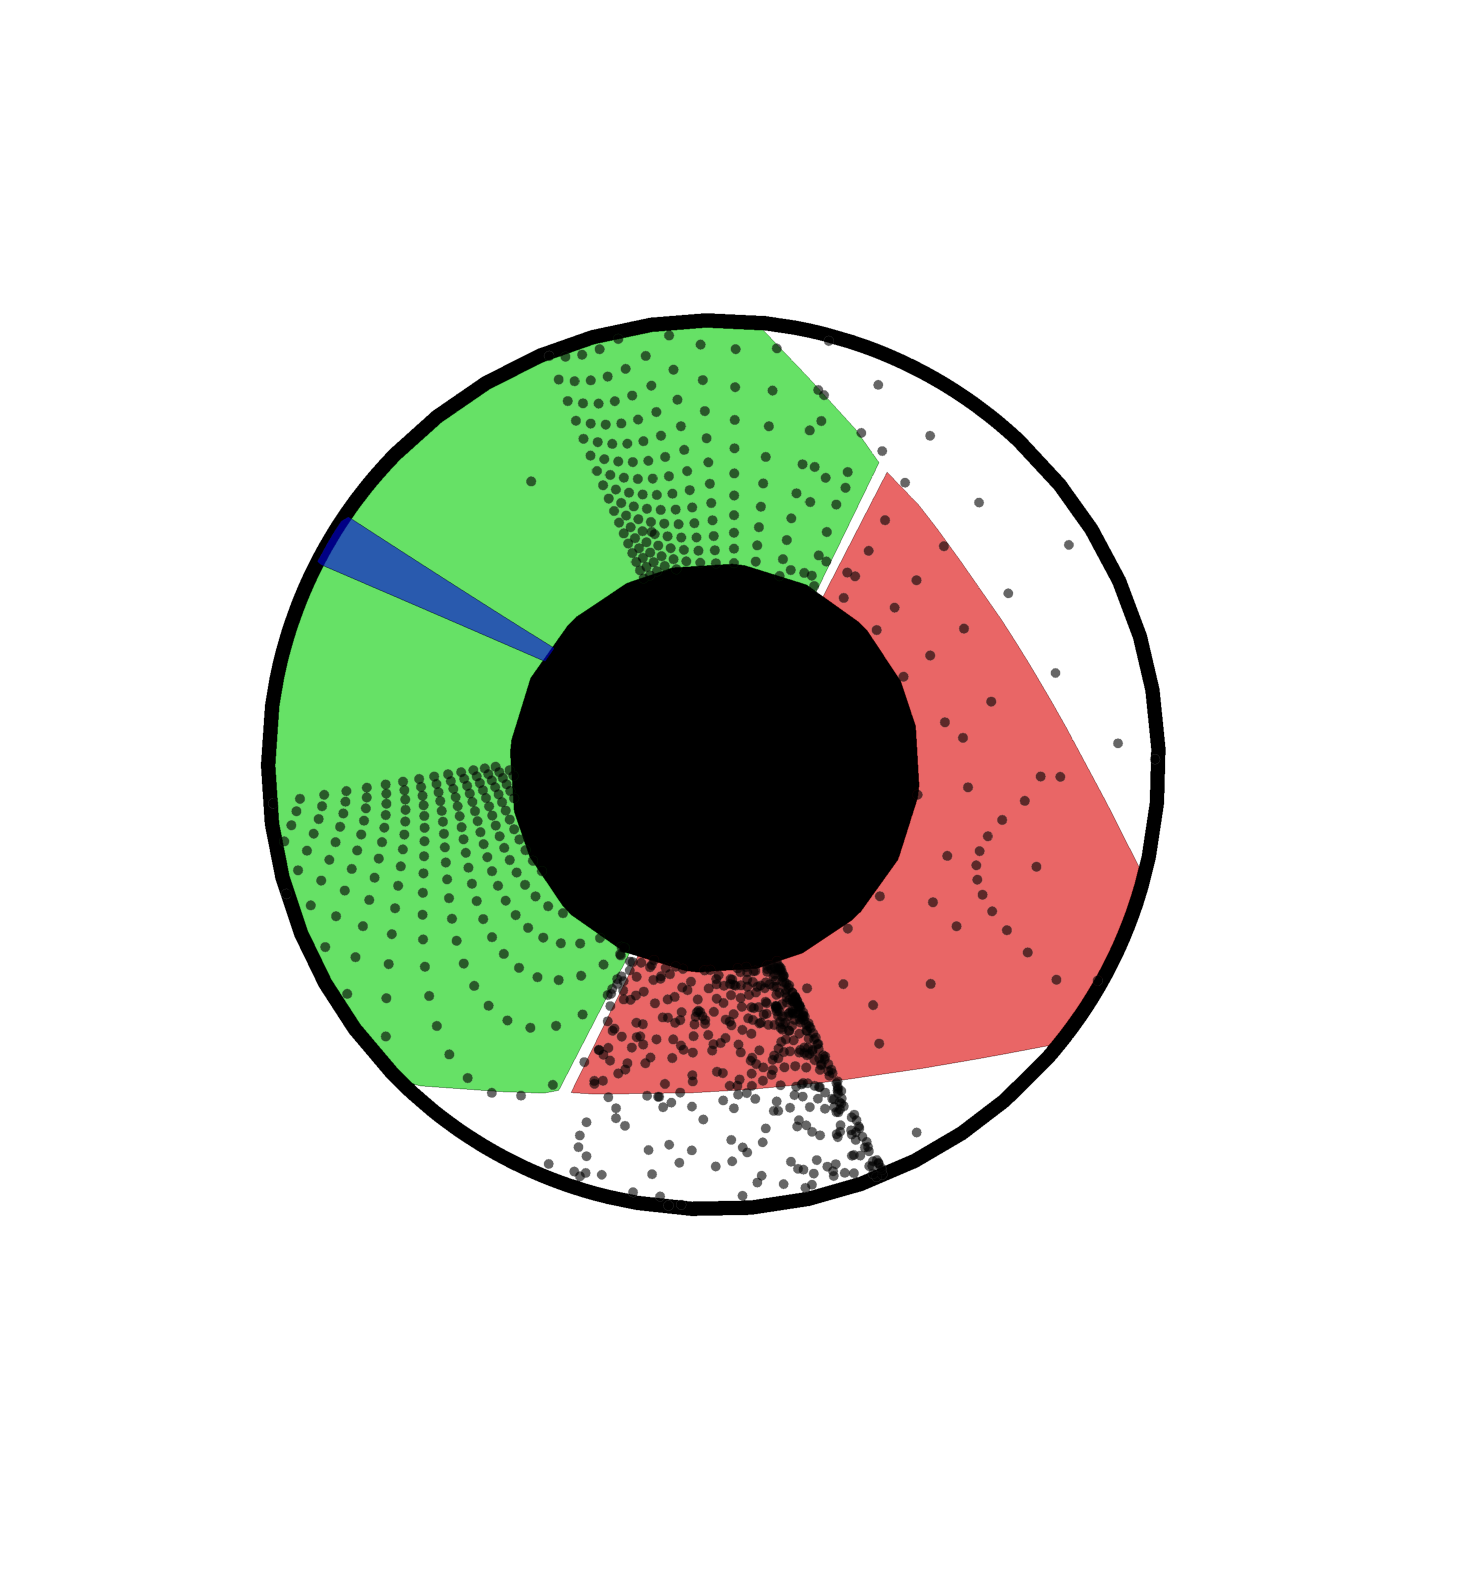
\includegraphics[width=.35\linewidth]{gfx/disk_cathegorization}} \quad
	{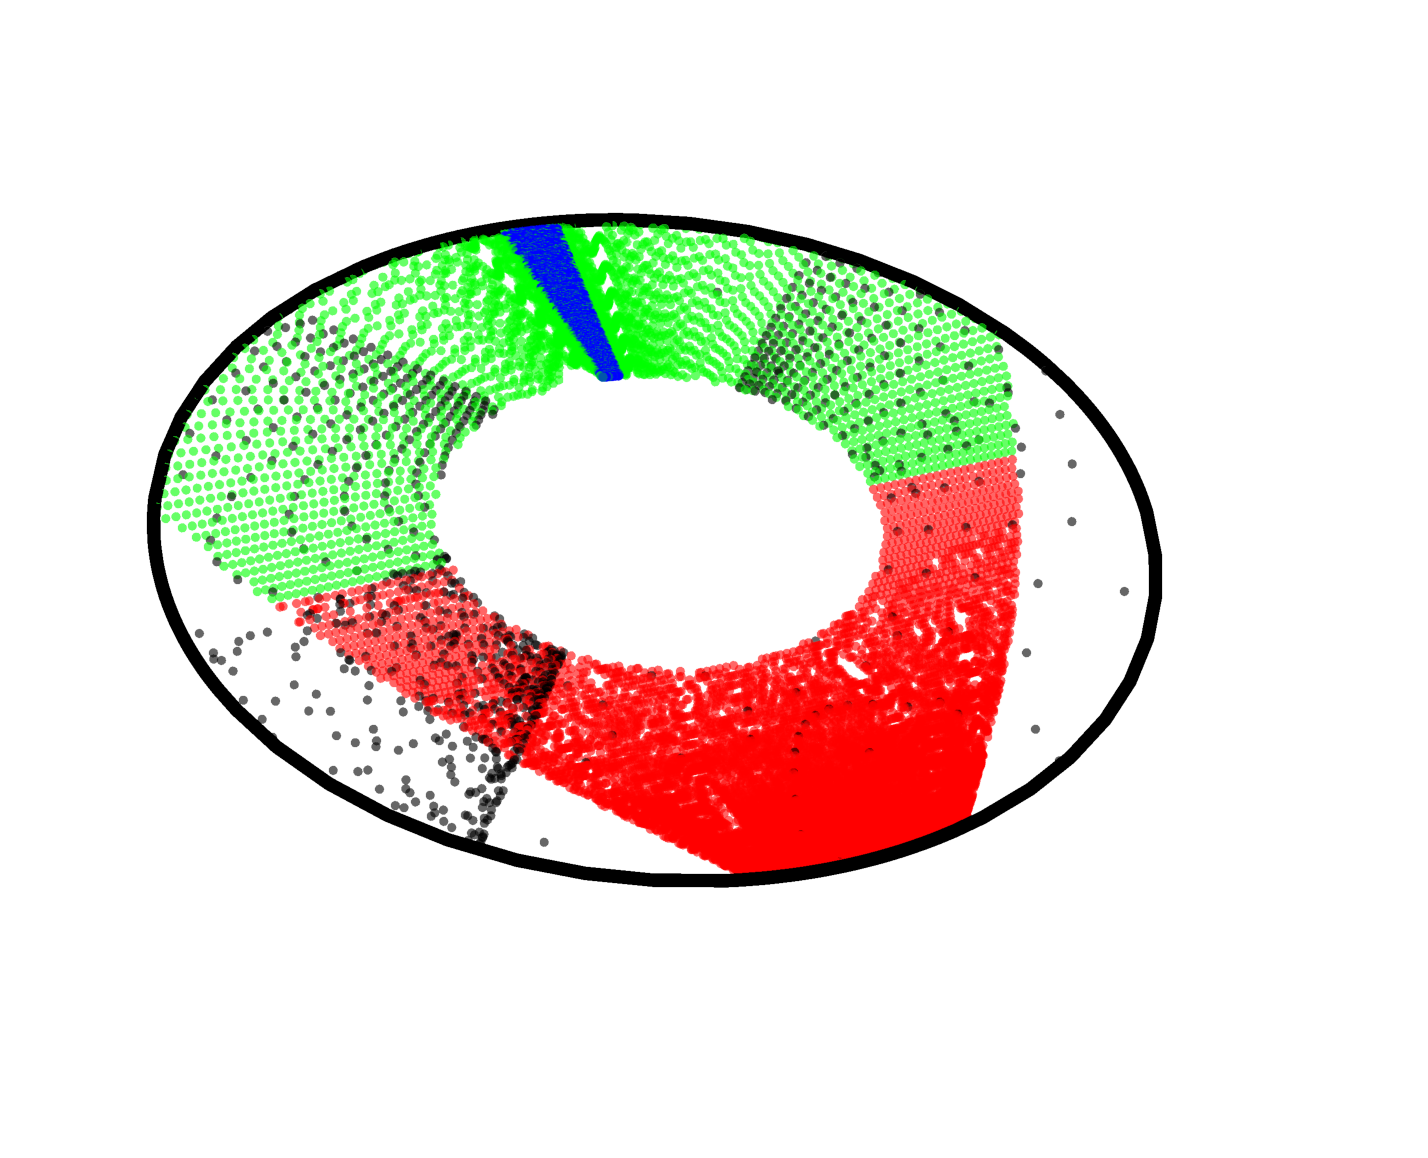
\includegraphics[width=.35\linewidth]{gfx/disk_cathegorization2}}
	\caption[Disk cathegorization]{Disk cathegorization.}
	\label{fig:cathegories}
\end{figure}

Finally, \autoref{fig:detail} shows a close up of the left side of the shadow where even more halos are appreciated. This time, for the sake of its beauty, a texture on the celestial sphere is added and the disk is drawn completely white.

\begin{figure}[bth]
	\myfloatalign
	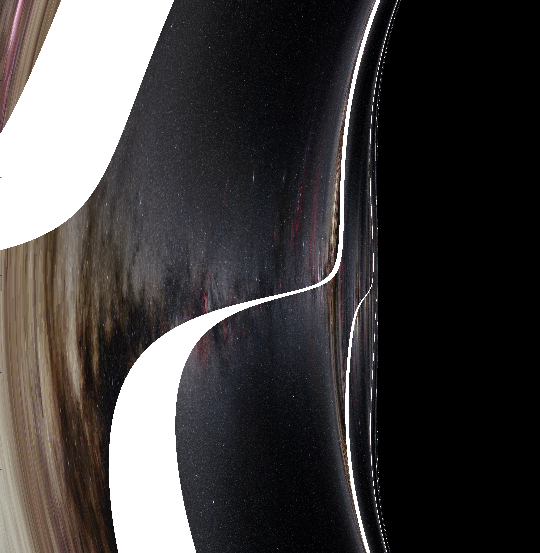
\includegraphics[width=.6\linewidth]{gfx/bh_detail_texture_disk-white}
	\caption[Close up of the shadow]{Close up of the shadow.}
	\label{fig:detail}
\end{figure}

\begin{figure}[bth]
	\myfloatalign
	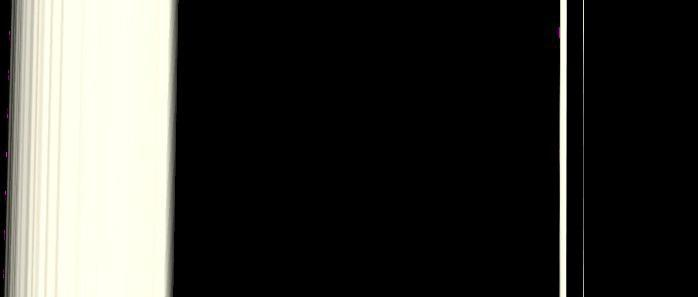
\includegraphics[width=.6\linewidth]{gfx/zoom}
	\caption[Zoom on the side of the shadow]{Zoom on the side of the shadow.}
\label{fig:zoom}
\end{figure}

\subsection{Infinite Images}

The previous study on the inner halo showed the first step to understand the infinite images of the disk we can see. Let us explain this with more detail: the shadow and the \ac{ISCO} are very close, so near the \ac{ISCO}, the particles turn around the black holes a great number of times. The previous study showed only the case where the particles make one full turn, but between that inner halo and the shadow there are an infinite number of halos.

Why an infinite number of images of the halo? For every turn completed by a geodesic, an image of the halo is generated near the black hole. That is, for every possible turn, a new image is generated.

This explains the infinite number of images, as the number of possible turns is, indeed, infinite. We can zoom even more to see more images of the same disk. 

\autoref{fig:zoom} shows two more halos between the studied halo and the shadow. The left big stripe on the left is what we called before inner halo. We see here that the term is not accurate, as there are more halos between it and the shadow. Greater zooms can be studied in order to see more images of the disk.

This property of the black holes deserves some more attention. A study on the shadow formation and geodesics near the \ac{ISCO} follows.

First of all, let us see \autoref{fig:virtualshadow}. This image depicts parallel geodesics that fall in the black hole. As we can see, the shadow seen on the right part of the image is much greater than the actual diameter of the black hole's horizon. This is due to the greatly curved spacetime, that forces even distant geodesics to curve and fall into the black hole. That way, the shadow is not the black hole's horizon, but the diameter for which the contained geodesics fall inside it.

We can study the \ac{ISCO} by studying geodesics that turn close to the horizon. \autoref{fig:isco} shows two examples of a set of geodesics on the equatorial plane that turn around the horizon once.

\begin{figure}[bth]
	\myfloatalign
	\subfloat[Horizon and shadow]
	{\label{fig:virtualshadow}
		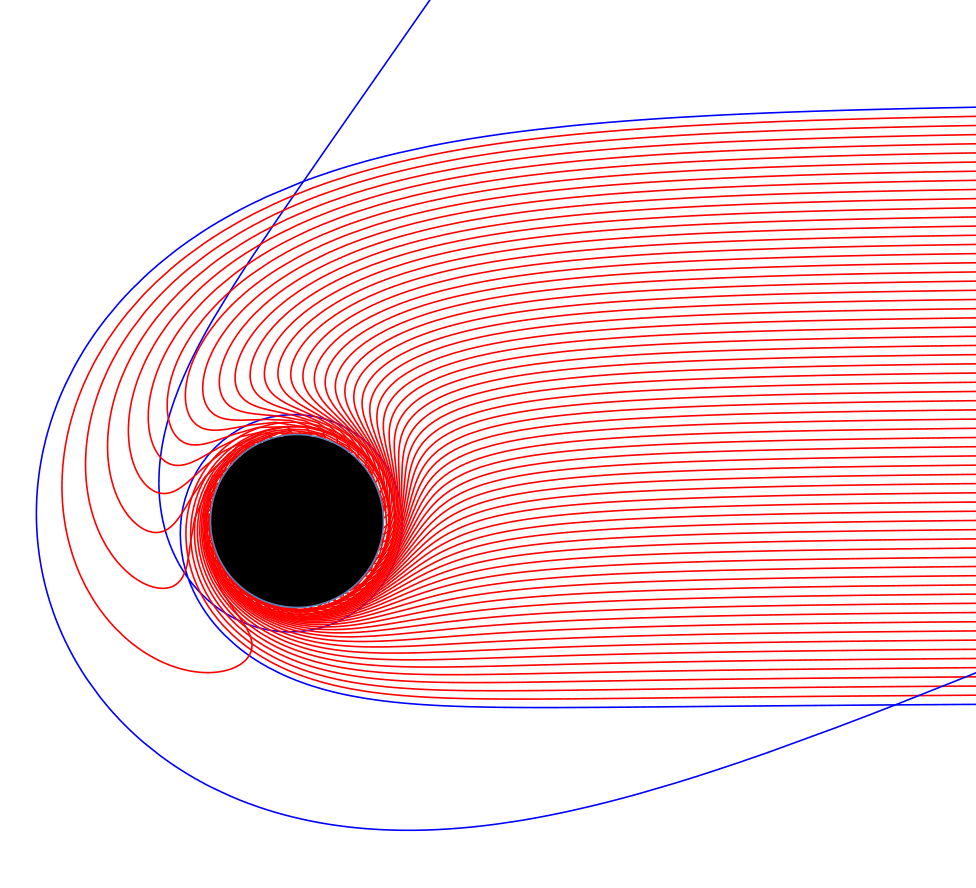
\includegraphics[width=.9\linewidth]{gfx/shadow}} \\
	{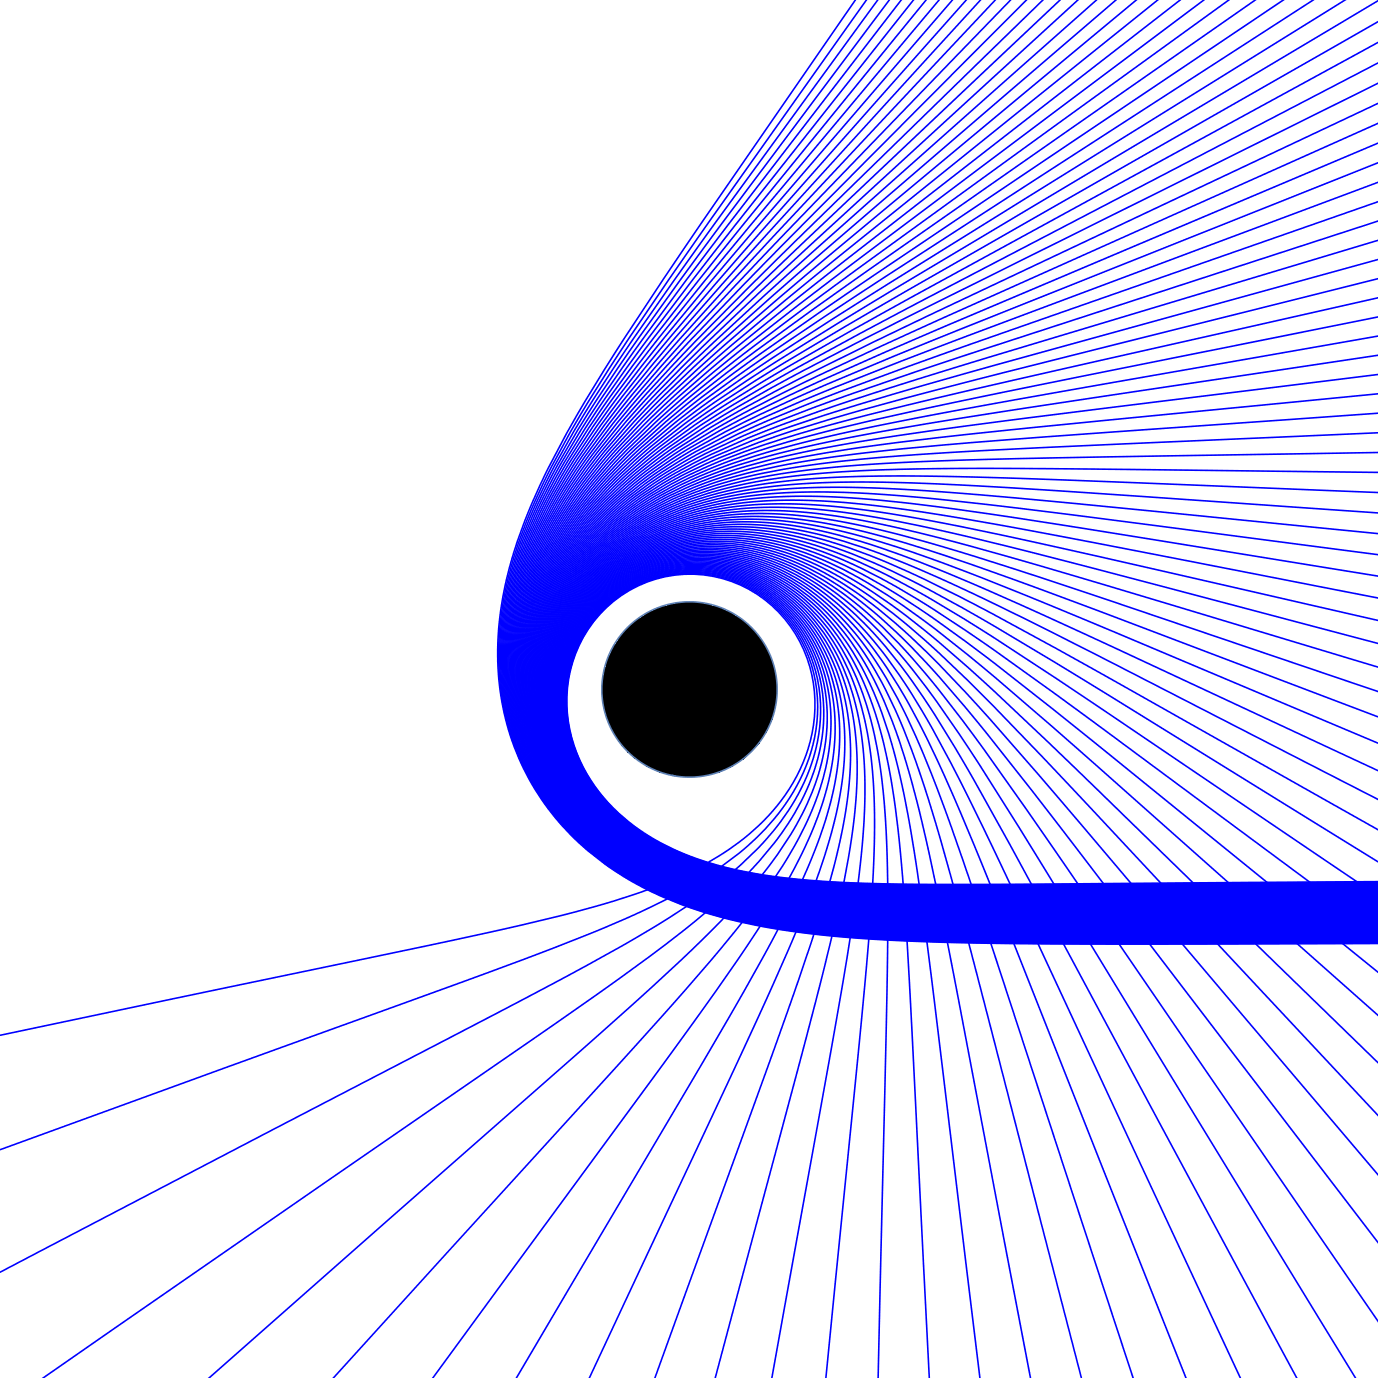
\includegraphics[width=.45\linewidth]{gfx/isco1}} \quad
	{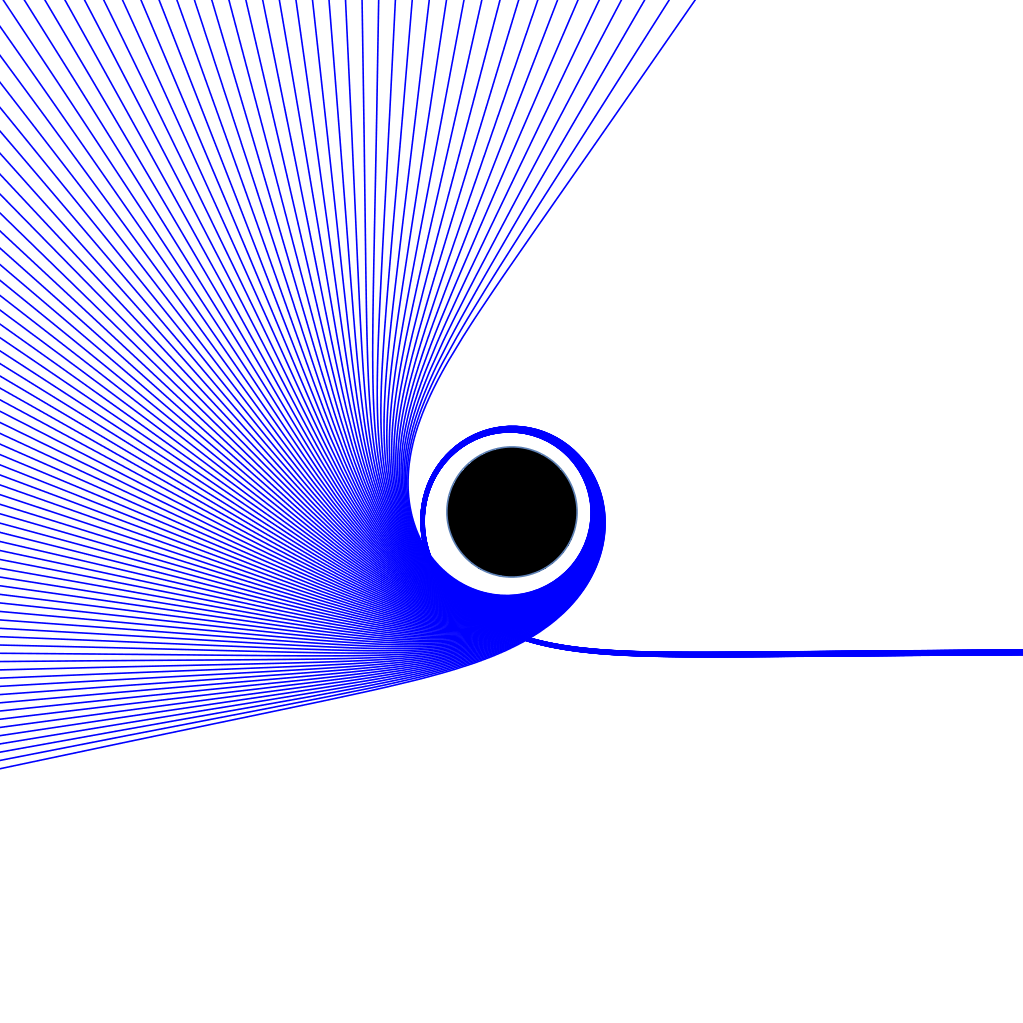
\includegraphics[width=.45\linewidth]{gfx/isco2}}
	\caption[Geodesics around the horizon]{Geodesics around the horizon.}
	\label{fig:isco}
\end{figure}

The number of turns a geodesic can make around the black hole, converging to the \ac{ISCO}, is arbitrary. \autoref{fig:isco4} shows a geodesic that turns up to four times around the black hole's horizon.

In fact, if the geodesic falls into the \ac{ISCO}, the number of turns is infinite, as shown on \autoref{fig:iscofinal}.

All this journey around the black hole explains why the number of images of the disk is infinite: as the geodesic can turn an arbitrary, and therefore infinite, number of times around the black hole, the disk will be infinitely repeated.

\begin{figure}[bth]
	\myfloatalign
	\subfloat[Geodesic turning four times]
	{\label{fig:isco4}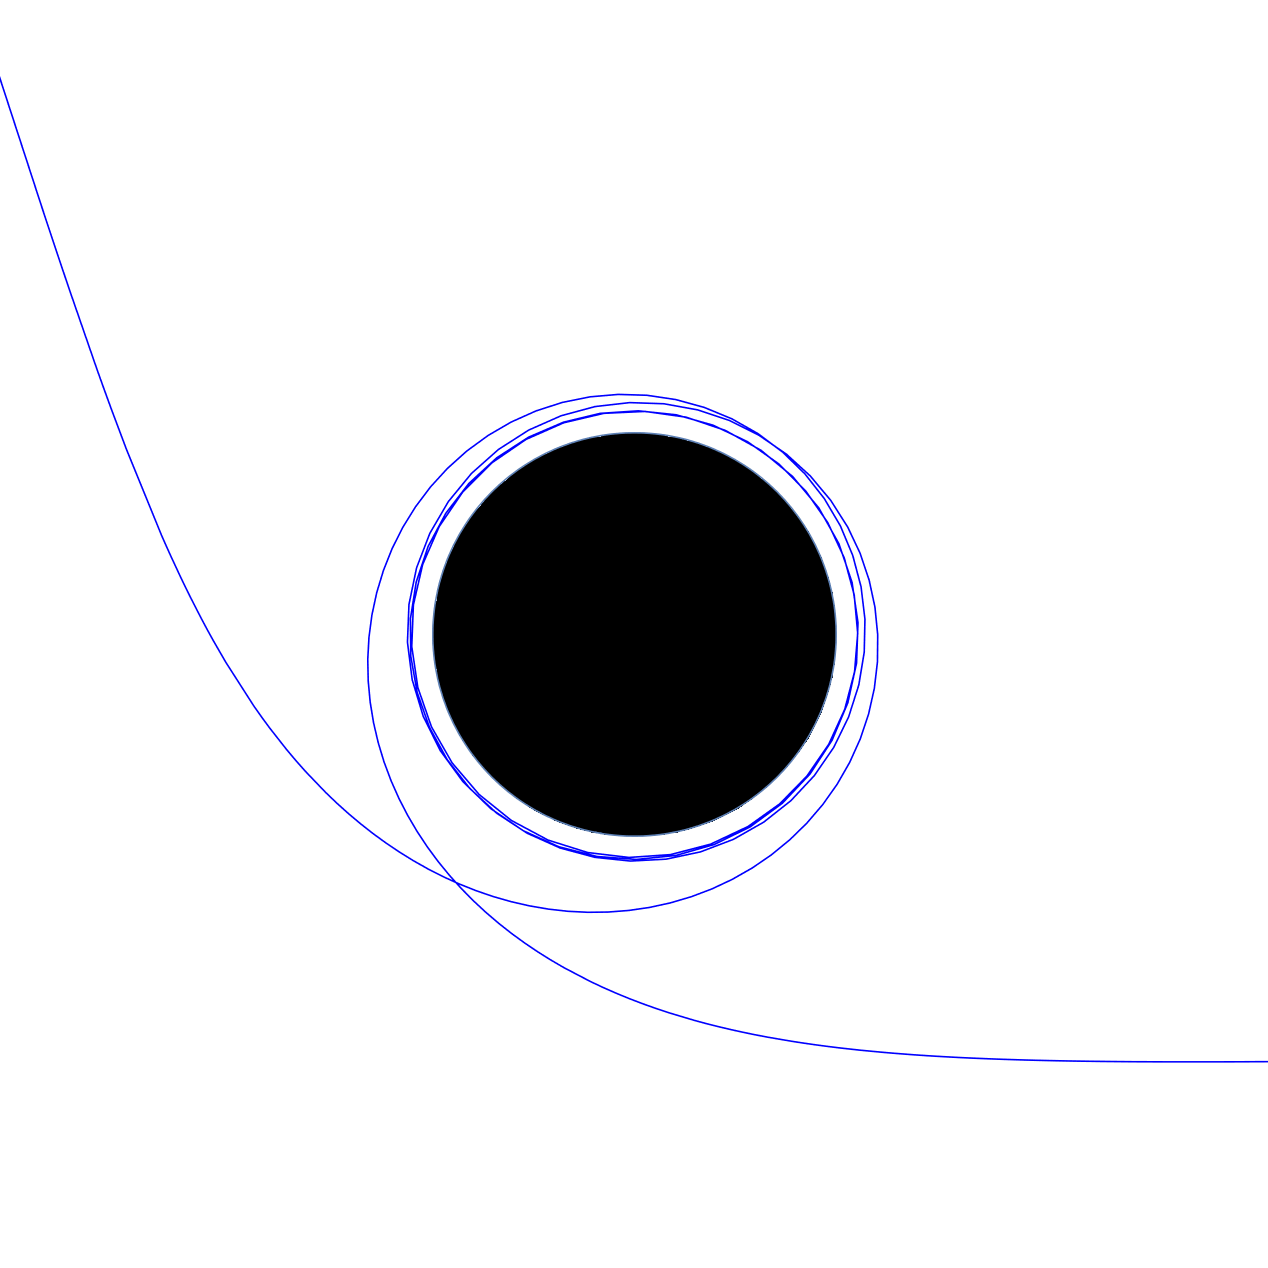
\includegraphics[width=.45\linewidth]{gfx/isco4}} \quad
	\subfloat[Geodesic falling into the ISCO]
	{\label{fig:iscofinal} 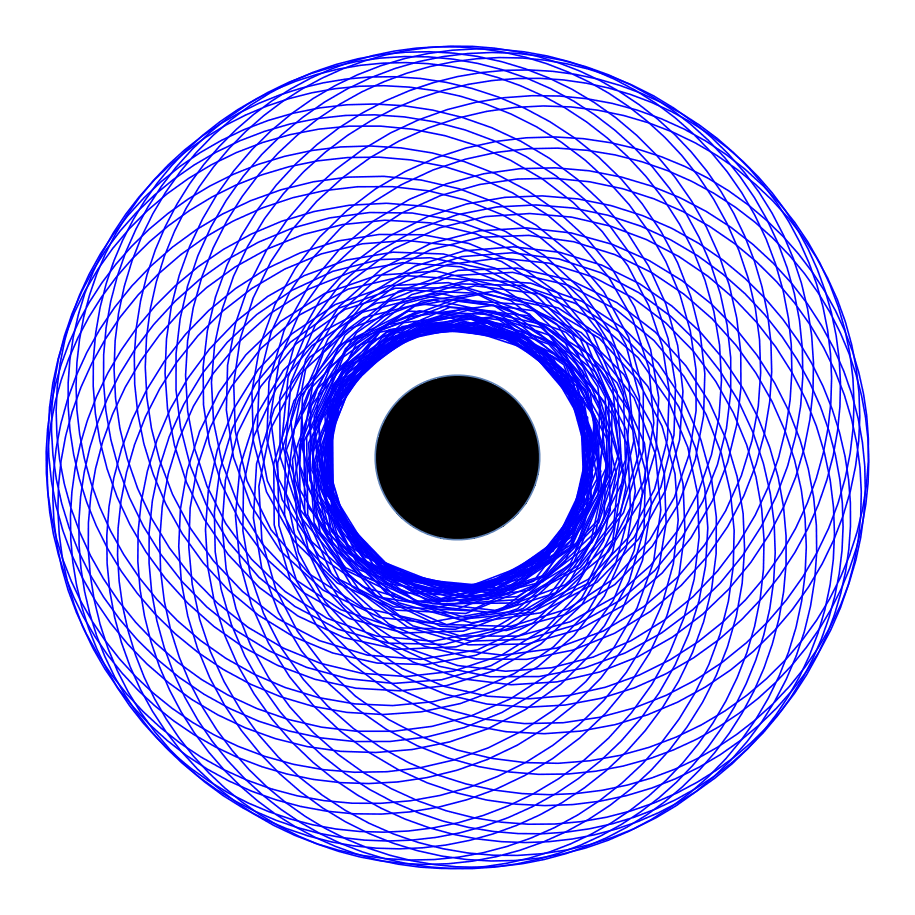
\includegraphics[width=.45\linewidth]{gfx/iscofinal}}
	\caption[Turning geodesics]{Turning geodesics.}
\end{figure}